% Author: Alfredo Sánchez Alberca (asalber@ceu.es)
%----------------------------------------------------------------------------------------
%    DOCUMENT CLASS
%----------------------------------------------------------------------------------------

\documentclass[11pt,a4paper,openright]{book}
%----------------------------------------------------------------------------------------
%	PACKAGES AND OTHER DOCUMENT CONFIGURATIONS
%----------------------------------------------------------------------------------------

% Language settings
\usepackage{polyglossia}
\setdefaultlanguage{english}

% Margins and layout
\usepackage[top=3cm, bottom=3cm, left=2.54cm, right=2.54cm]{geometry}

% Font settings
\usepackage{fontspec}
\setmainfont[Ligatures=TeX]{TeX Gyre Pagella}
\usepackage{unicode-math}
\setmathfont[math-style=ISO,bold-style=ISO,vargreek-shape=TeX]{TeX Gyre Pagella Math}

% Color
\usepackage{xcolor} % Required for specifying colors by name
\definecolor{color1}{RGB}{5,161,230}
\definecolor{color2}{RGB}{238,50,36}
\definecolor{ocre}{RGB}{243,102,25} % Define the orange color used for highlighting throughout the book
\definecolor{blueceu}{RGB}{5,161,230} % Blue color of CEU logo
\definecolor{greenceu}{RGB}{185,209,16} % Green color of CEU logo
\definecolor{redceu}{RGB}{238,50,36} % Red color of CEU logo
\definecolor{grayceu}{RGB}{111,107,83} % Gray color of CEU logo
\definecolor{coral}{rgb}{1,0.5,0.31} % Orange color for graphics
\definecolor{royalblue1}{rgb}{0.28,0.46,1} % Blue color for graphics
\definecolor{mygreen}{rgb}{0,0.8,0} % Green color for graphics
\definecolor{chaptergrey}{RGB}{5,161,230} % Blue color of CEU logo

% Math support
\usepackage{amsmath} 

% Line breaking
\usepackage{microtype} 
\setlength{\emergencystretch}{2em}

% Graphics
\usepackage{graphicx}
\usepackage{tikz} 
\usepackage{eso-pic} % Required for specifying an image background in the title page

% Arrays and tables
\usepackage{array}
\usepackage{multirow}
\usepackage{colortbl}
\usepackage{booktabs}
\newcommand{\tcrule}{\arrayrulecolor{color1!50!white}\toprule}
\newcommand{\mcrule}{\arrayrulecolor{color1!50!white}\midrule}
\newcommand{\bcrule}{\arrayrulecolor{color1!50!white}\bottomrule}

% Captions
\usepackage[margin=20pt, font=small, labelfont=bf, labelsep=endash]{caption}

% Floating figures
\usepackage{subfigure}

% Lists
\usepackage[shortlabels]{enumitem} % Customize lists
%\setlist{nolistsep} % Reduce spacing between bullet points and numbered lists
\setlist[description]{style=sameline,leftmargin=0cm}

\makeatletter
\let\savees@listquot\es@listquot
\def\es@listquot{\protect\savees@listquot}
\makeatletter

\renewcommand{\theenumiii}{\arabic{enumiii}}

% Flush floating 
\usepackage{afterpage}

% Creative common icons
\usepackage[scale=2]{ccicons}

% hyperlinks
\usepackage{hyperref}
\hypersetup{
pdfauthor = {Alfredo S\'anchez Alberca},
pdftitle = {Applied Biostatistics with R},
pdfsubject = {Biostatistics},
pdfkeywords = {Statistics, Biostatistics, R},
pdfcreator = {XeLaTeX with hyperref package},
pdfproducer = {pdfLaTeX},
colorlinks = true,
linkcolor = red,          % color of internal links
citecolor = green,        % color of links to bibliography
filecolor = magenta,      % color of file links
urlcolor = magenta,          % color of external links
}
%\usepackage{breakurl}

% Indentation
%\setlength\parindent{0pt}

% Control of widow orphan lines
\clubpenalty=10000
\widowpenalty=10000 

%Code listing formatting
\usepackage{listings}
\lstdefinelanguage{morejava}{morekeywords={String}}
\definecolor{vollgrau}{rgb}{0.9,0.9,0.9}
\definecolor{colKeys}{rgb}{0,0,1}
\definecolor{colIdentifier}{rgb}{0,0,0}
\definecolor{colComments}{rgb}{1,0.5,0}
\definecolor{colString}{rgb}{0,0.5,0}
\definecolor{colbackground}{rgb}{0.9,0.9,1}
\lstset{%
     language=R,
     float=hbp,%
     basicstyle=\ttfamily,%
     identifierstyle=\color{colIdentifier},%
     keywordstyle=\color{colKeys},%
     stringstyle=\color{colString},%ROMERO OTERO, JAVIER
     commentstyle=\color{colComments},%
%    columns=flexible,%
%    columns=fullflexible,%
     columns=fixed,
     tabsize=1,%
     extendedchars=true,%
     showspaces=false,%
     showstringspaces=false,%
     breaklines=true,%
     breakindent=10pt,%
     backgroundcolor=\color{colbackground},%
     breakautoindent=true,%
     captionpos=t,%
     xleftmargin=1em,%
%    xrightmargin=.5\fboxsep,%
     numbersep=1em,%
     escapechar=\#
}

% Set short or long depending on the version desired
% \usepackage[corto]{optional}

\input{preamble/commands_book} % Insert the commands_book.tex file which contains the majority of the structure behind
% the template

%----------------------------------------------------------------------------------------
%	COMMANDS FOR INDICATIONS
%----------------------------------------------------------------------------------------
\usepackage{menukeys}
\newmenucolortheme{mycolors}{named}{white}{color1}{black}
\changemenucolortheme{menus}{mycolors}
\renewmenumacro{\menu}[>]{menus}
%\newmenustylesimple*{botonstyle}{\textbf{\CurrentMenuElement}}
%\renewmenumacro{\keys}{botonstyle}
\newcommand{\button}[1]{\textsf{\small #1}}
\newcommand{\option}[1]{\textsf{\small #1}}
\newcommand{\mtab}[1]{\textsf{\small #1}}
\newcommand{\field}[1]{\textsf{\small #1}}
\newcommand{\command}[1]{\texttt{#1}}
\newcommand{\variable}[1]{\textsf{\small #1}}
\newcommand{\result}[1]{\texttt{#1}}

% OTHERS
\newcommand{\resetcounters}{\setcounter{page}{1} \setcounter{section}{0} \setcounter{footnote}{0} \setcounter{figure}{0} \setcounter{table}{0}}


%========================================================================================
%   DOCUMENT BODY
%========================================================================================
\begin{document}
\frontmatter 
% Add two blank pages at the begining
%\null\thispagestyle{empty}\newpage
%\null\thispagestyle{empty}\newpage
%----------------------------------------------------------------------------------------
%	TITLE PAGE
%----------------------------------------------------------------------------------------
\begin{titlepage}
\thispagestyle{empty}
\vspace*{7cm}
\par

% Book title
\begin{center}
\normalfont\fontsize{30}{30}\selectfont
{\bfseries \color{blueceu}Applied Biostatistics\\ with R and rk.Teaching}
\end{center}
\vspace{1cm}

% Authors names
\begin{center}
\Large
\begin{tabular}{c}
Edgar Arribas Gimeno (\url{edgar.arribasgimeno@ceu.es})\\
Juan Carlos Garro Garro (\url{garro.eps@ceu.es})\\
Alfredo Sánchez Alberca (\url{asalber@ceu.es})\\
Alberto Zaragoza de Lorite (\url{alberto.zaragozalorite@ceu.es})
\end{tabular}

\medskip 
Department of Maths and Data Science\\ CEU San Pablo\\[1cm]
\medskip 
September 2022

\vspace{1cm}
\includegraphics[height=3cm]{img/logo_uspceu}
\end{center}
\vfill
\end{titlepage} 
%\input{preamble/titlepage_book} 
 
%----------------------------------------------------------------------------------------
%	COPYRIGHT PAGE
%----------------------------------------------------------------------------------------
\input{preamble/license}

%----------------------------------------------------------------------------------------
%	TABLE OF CONTENTS
%----------------------------------------------------------------------------------------
%\chapterimage{img/chapter_head.png} % Table of contents heading image
{\pagestyle{plain} % No headers
%\input{registro}
\tableofcontents\thispagestyle{empty}
  % Print the table of contents itself
\cleardoublepage % Forces the first chapter to start on an odd page so it's on the right
}

\mainmatter 
%----------------------------------------------------------------------------------------
%	CHAPTERS 
%----------------------------------------------------------------------------------------
% % Author: Alfredo Sánchez Alberca (asalber@ceu.es)

\chapter{Introduction to R and RKWard}\label{cha:introduction}

\section{Introduction}
The big computing power achieved by computers has made them powerful tools essentials for all those disciplines, such as
Statistics, that require managing large volumes of data.
Nowadays, nobody addresses a serious statistical study without the help of data analysis software. 

\emph{R} is a powerful programming language that includes a lot of functions for representing and analyzing data. 
It was developed by Robert Gentleman and Ross Ihaka at the university of Auckland in New Zealand, although now is
maintained by a large scientific community all around the world.

\begin{center}

\includegraphics[scale=0.5]{chapters/introduction/img/Rlogo}
\end{center} 

The advantages of R with respect to other data analysis software like SPSS, SAS, Matlab, Minitqab or Excel, are
multiple:
\begin{itemize}
\item It's open source software, what implies that it's free. 
It can be downloaded from the web \url{http://www.r-project.org/}.
\item It's multi-platform .
There are versions for the main platforms: Windows, Macintosh, Linux, etc. 
\item It's supported by a huge scientific community that uses the software as an standard for data analysis. 
\item It has thousands of packages for performing any type of data analysis and graphics representations, from the most
common to the most innovative and cutting edge statistical procedures that are not included in other software. 
The packages are organized and documented in the CRAN (Comprehensive R Archive Network) repository, from where they
can be downloaded for free. 
In Spain there is a mirror of this repository in the web \url{http://cran.es.r-project.org/}.
\item It's programmable, what means that the user can create easily their own functions or packages for specific data
analysis.
\item There are a lot of books, manuals and tutorials for free, that allow the learning even for advances uses
in all kind of disciplines like Mathematics, Physics, Chemistry, Biology, Psychology, Medicine, etc. 
\end{itemize}

By default the working environment of R is the command line, what means that the computations are done with commands
manually typed in a text window.
However, there exists some graphical user interfaces (GUI) that ease its use, particularly for newbies.
The GUI that we are going to use along these practices is \emph{RKWard}, developed by Thomas
Friedrichsmeier, and the package rk.Teaching developed by Alfredo Sánchez Alberca in the CEU San Pablo
University and specifically designed for teaching Statistics.

\begin{center}
  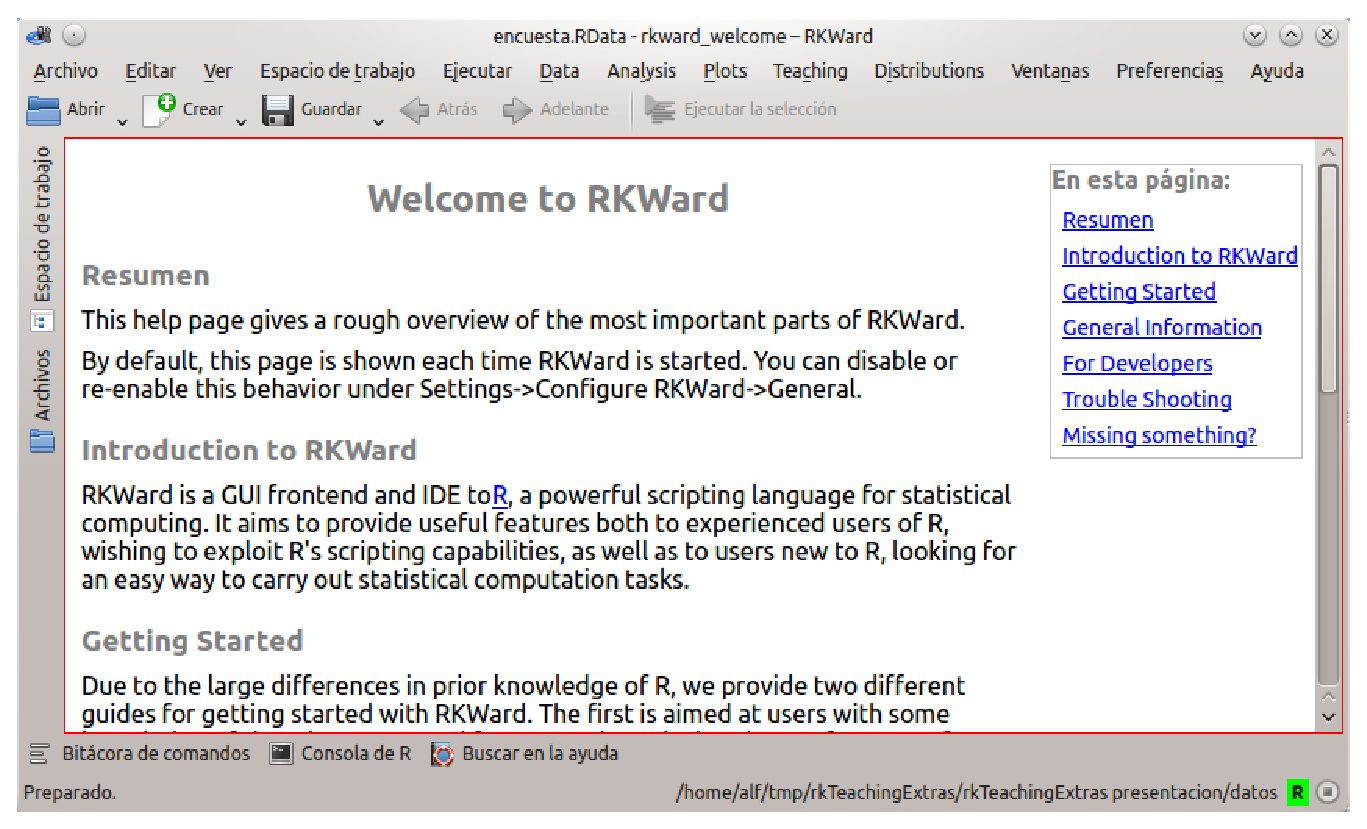
\includegraphics[width=\textwidth]{chapters/introduction/img/rkward}
\end{center}

The main goal of this chapter is to introduce the student to the use of RKWard and rk.Teaching, showing him the basic
operations to enter and manipulate data.

\section{Installation}
The installation of the required software for these practices depends on the operating system.

\subsection{Windows}
For Windows there is an installation bundle that included R, RKWard and rkTeaching. The installation program can be downloaded from \url{https://aprendeconalf.es/en/project/rkteaching/#installation-on-windows}.

\subsection{MacOs}
For MacOs, R must be installed first, after RKWard and finally the package rkTeaching. The steps to do the installation are described at \url{https://aprendeconalf.es/en/project/rkteaching/#installation-on-mac-os}.

\subsection{Linux}
For Linux, R must be installed first, after RKWard and finally the package rkTeaching. The steps to do the installation are described at \url{https://aprendeconalf.es/en/project/rkteaching/#installation-on-linux}.


\section{Solved exercises}
\begin{enumerate}[leftmargin=*]
\item Create a data set with the data in the sample below and save it with name \variable{colesterol.rda}
\begin{center}
\begin{tabular}{|l|c|r|r|r|}
\hline
\multicolumn{1}{|c|}{Name} & \multicolumn{1}{c|}{Gender} & \multicolumn{1}{c|}{Weight} & \multicolumn{1}{c|}{Height} &
\multicolumn{1}{c|}{Cholesterol}\\
\hline
José Luis Martínez Izquierdo  & M &  85 & 179 & 182\\
Rosa Díaz Díaz & F & 65 & 173 & 232\\
Javier García Sánchez  & M & 71 & 181 & 191\\
Carmen López Pinzón & F &  65 & 170 & 200\\
Marisa López Collado & F &  51 & 158 & 148\\
Antonio Ruiz Cruz & M & 66 & 174 & 249\\
\hline
\end{tabular}
\end{center}

\begin{indication}
To create a data set:
\begin{enumerate}
\item Select the menu \menu{File > New > Dataset}.
\item In the dialog displayed enter the name \variable{cholesterol} and click the button \button{OK}.
\item In the data editor window, define a variable in every column giving a name for the variable in the \field{Name}
row, a type (Numeric, Factor, String or Logical) in the \field{Type} row, and in the case of a factor, defining its
levels in the \field{Levels} row.
\item After define the variable, enter the data of every variable in the sample in the corresponding column.
\end{enumerate}
To save the data set:
\begin{enumerate}
\item Select the menu \menu{Workspace > Save Workspace}.
\item In the dialog displayed give the name \variable{cholesterol.rda} to the file, select the folder where to save it
and click the button \button{Save}.
\end{enumerate}
\end{indication}

\item Define a new variable \variable{Age} with the ages of the individuals in the sample, between the variables
\variable{Name} and \variable{Gender}.
\begin{center}
\begin{tabular}{|l|r|}
\hline
\multicolumn{1}{|c|}{Name} & \multicolumn{1}{c|}{Age} \\
\hline
José Luis Martínez Izquierdo & 18 \\
Rosa Díaz Díaz & 32 \\
Javier García Sánchez & 24 \\
Carmen López Pinzón & 35 \\
Marisa López Collado & 46 \\
Antonio Ruiz Cruz & 68 \\
\hline
\end{tabular}
\end{center}

\begin{indication} 
\begin{enumerate}
\item Click the left tab \button{Workspace}.
\item In the workspace window double-click the data set \variable{cholesterol} to edit it.
\item In the data editor window, right-click the column header of the variable \variable{Gender} and select
\menu{Insert new variable left}. 
\item In the new empty column enter the name and type of the variable \variable{Age}, and enter the age of every
individual.
\end{enumerate}
\end{indication}

\item Insert the following data of a new individual:
\begin{quote}
Name: Cristóbal Campos Ruiz.\\
Age: 44 years.\\
Gender: Male.\\
Weight: 70 Kg.\\
Height: 178 cm.\\
Cholesterol: 220 mg/dl.
\end{quote}

\begin{indication}
\begin{enumerate}
\item Insert the data of the new individual in the first empty row.
\end{enumerate}
\end{indication}

\item Create a new variable with the body mass index of every individual using the formula
\[
\text{bmi} = \frac{\text{Weight (in Kg)}}{\text{Height (in m)}^2}
\]

\begin{indication}
\begin{enumerate}
\item Select the menu \menu{Teaching > Data > Compute variable}.
\item In the dialog displayed enter the formula to compute the body mass index in the field \field{Variable
computation}.
\item In the field \field{Save as} click the button \button{Change}.
\item In the dialog displayed select as a parent object the data set \variable{cholesterol} and click
the button \button{OK}.
\item Enter the name \variable{bmi} for the new variable and click the button \button{Submit}.
\end{enumerate}
\end{indication}

\item Recode the body mass index variable into a new categorical variable \variable{Obesity} according to the following
rules:
\begin{center}
\begin{tabular}{lcl}
Less than de $18.5$ & \rightarrow & Low weight\\
From $18.5$ to $24.5$ & \rightarrow & Healthy\\
From $24.5$ to $30$ & \rightarrow & Overweight\\
Greater than $30$  & \rightarrow & Obese
\end{tabular}
\end{center}

\begin{indication}
\begin{enumerate}
\item Select the el menu \menu{Teaching > Data > Variable recoding}.
\item In the dialog displayed insert the variable \variable{bmi} in the field \field{Variable to recode}.
\item Enter the recoding rules below in the field \field{Recoding rules}:
\begin{quote}
\lstinline{lo:18.5 = 1}\\
\lstinline{18.5:24.5 = 2}\\
\lstinline{24.5:30 = 3}\\
\lstinline{30:hi = 4}
\end{quote}
\item In the field \field{Save as} click the button \button{Change}.
\item In the dialog displayed select as a parent object the data set \variable{cholesterol} and click the button
\button{OK}.
\item Enter the name \variable{Obesity} for the new variable and click the button \button{Submit}.
\item In the data edition window, enter the levels for the \variable{Obesity} factor, setting the label ``Low weight''
for the first category, ``Healthy'' for the second one, ``Overweight'' for the third and ``Obese'' for the fourth.
\end{enumerate}
\end{indication}


\item Filter the data set to get a new data set with the data of males. 
\begin{indication}
\begin{enumerate}
\item Select the menu \menu{Teaching > Data > Data filtering}.
\item In the dialog displayed insert the data set \variable{cholesterol} in the field \field{Data set}.
\item Insert the expression \lstinline{gender=="M"} in the field \field{Selection condition}.
\item Enter the name \variable{cholesterol.males} for the new data set and click the button \button{Submit}.
\end{enumerate}
\end{indication}

\end{enumerate}

\section{Proposed exercises}
\begin{enumerate}[leftmargin=*]
\item The data set \variable{neonates} of the package \variable{rk.Teaching}, contains information about a
sample of 320 newborns that meet the normal gestation time in a hospital during one year.
Do the following operations:
\begin{enumerate}
\item Load the data set.
\begin{indication}
\begin{enumerate}
\item Click the \field{Workspace} tab and double-click the \variable{rk.Teaching} package to unfold the data sets that
it contains. 
\item Right-click the data set \variable{nenonates} and select the menu \menu{Copy to .GlobalEnv} to copy the data
set to the working environment.
\end{enumerate}
\end{indication}

\item Compute the variable \variable{APGAR.average} as the mean of the variables \variable{APGAR1} and
\variable{APGAR5}.
\item Recode the variable \variable{weight} into the factor \variable{weight.category} with two categories
corresponding to weights less than and greater than $2.5$ Kg.
\item Recode the variable \variable{APGAR1} into the factor \variable{APGAR.state} with three categories: depressed
(APGAR$\leq 3$), moderately depressed ($3<$APGAR$\leq 6$) and normal (APGAR$>6$).
\item Filter the data set to get a new data set with the neonates of non-smoking mothers with an APGAR score at 1
minute less than or equal to 3.
How many neonates are there?
\end{enumerate}
\end{enumerate}

% Author: Alfredo Sánchez Alberca (asalber@ceu.es)

\chapter{Frequency distributions and charts}\label{cha:freqency-distributions}

\section{Solved exercises}
\begin{enumerate}[leftmargin=*]

\item The number of children in a sample of 25 is
\begin{center}
1, 2, 4, 2, 2, 2, 3, 2, 1, 1, 0, 2, 2, 0, 2, 2, 1, 2, 2, 3, 1, 2, 2, 1, 2.
\end{center}
Do the following operations:
\begin{enumerate}
\item Create a data frame with the variable \variable{children} and enter the data.

\item Create the frequency table.
\begin{indication}
\begin{enumerate}
\item Select the menu \menuc{Teaching > Frequency distribution > Frequency tabulation} .
\item In the dialog displayed, select the variable \variable{children} in the field \field{Variable to tabulate} and
click the button \button{Send}.
\end{enumerate}
\end{indication}

\item Create the absolute frequency bar chart.
\begin{indication}
\begin{enumerate}
\item Select the menu \menu{Teaching > Charts > Bar chart}.
\item In the dialog displayed, select the variable \variable{children} in the field \field{Variable} and click
the button \button{Send}.
\end{enumerate}
\end{indication}

\item Create also the relative frequency, cumulative absolute frequency and cumulative relative frequency bar charts,
with their respective polygons.
\begin{indication}Follow the steps above checking, in the \option{Bar options} tab, the box
\option{Relative frequencies} for the relative frequencies bar chart, the box \option{Cumulative
frequencies} for the cumulative absolute bar chart, and both of them for the cumulative relative frequency bar chart. 
Check the box \option{Polygon}, to plot the corresponding polygon. 
\end{indication}
\end{enumerate}

\item The number of people treated in the emergency service of a hospital every day of November was
\begin{center}
15 \quad 23 \quad 12 \quad 10 \quad 28 \quad 7 \quad 12 \quad 17 \quad 20 \quad 21 \quad 18 \quad 13 \quad 11 \quad 12 \quad 26 \\
30 \quad 6 \quad 16 \quad 19 \quad 22 \quad 14 \quad 17 \quad 21 \quad 28 \quad 9 \quad 16 \quad 13 \quad 11 \quad 16 \quad 20
\end{center}
Do the following operations: 
\begin{enumerate}
\item Create a data frame with the variable \variable{emergencies} and enter the data.

\item Create the box plot. Are there some outlier? In that case, remove the outliers and proceed with the next part.
\begin{indication}
\begin{enumerate}
\item Select the menu \menu{Teaching > charts > Box plot}.
\item In the dialog displayed select the variable \variable{emergencies} in the field \field{Variables} and
click the button \button{Send}.
\item In the output windows with the box plot identify the outliers.
\item In the data frame edition tab, remove the rows with the outliers right-clicking the row header and selecting
\menu{Delete this row}.
\end{enumerate}
\end{indication}

\item Create the frequency table grouping data into 5 classes.
\begin{indication}
\begin{enumerate}
\item Select the menu \menu{Teaching > Frequency distribution > Frequency tabulation}.
\item In the dialog displayed select the variable \variable{emergencies}.
\item In the \option{Classes} tab check the box \option{Grouping intervals}, check the option \option{Number of
intervals}, enter the desired number of intervals in the field \field{Suggested intervals} and
click the button \button{Send}.
\end{enumerate}
\end{indication}

\item Create the absolute frequencies histogram.
\begin{indication}
\begin{enumerate}
\item Select the menu \menu{Teaching > charts > Histogram}.
\item In the dialog displayed select the variable \variable{emergencies} in the field \field{Variable}.
\item In the \option{Classes} tab, check the box \option{Grouping intervals}, check the box
\option{Number of intervals}, enter the desired number of intervals in the field \field{Suggested intervals} and click
the button \button{Send}.
\end{enumerate}
\end{indication}

\item Create also the relative frequency, cumulative absolute frequency and cumulative relative frequency
histograms, with their respective polygons.
\begin{indication}Follow the steps above checking, in the \option{Histogram options},
the box \option{Relative frequencies} for the relative frequency histogram, the box \option{Cumulative frequencies} for
the cumulative absolute frequency histogram, and both of them for the cumulative relative frequency histogram.
Check the box \option{Polygon} to plot the corresponding polygon. 
\end{indication}
\end{enumerate}

\item The blood type of a sample of 30 persons are:
\begin{center}
A, B, B, A, AB, 0, 0, A, B, B, A, A, A, A, AB,\\
A, A, A, B, 0, B, B, B, A, A, A, 0, A, AB, 0. 
\end{center}
Do the following operations:
\begin{enumerate}
\item Create a data frame with the variable \variable{blood.type} and enter the data.

\item Create the frequency table.
\begin{indication}
\begin{enumerate}
\item Select the menu \menu{Teaching > Frequency distribution > Frequency tabulation}.
\item In the dialog displayed, select the variable \variable{blood.type} in the field
\field{Variable to tabulate} and click the button \button{Send}.
\end{enumerate}
\end{indication}

\item Create the pie chart.
\begin{indication}
\begin{enumerate}
\item Select the menu \menu{Teaching > charts > Pie chart}.
\item In the dialog displayed, select the variable \variable{blood.type} in the field \field{Variables} and click the
button \button{Send}.
\end{enumerate}
\end{indication}
\end{enumerate}

\item The age and the marital status of a sample of 27 persons are:
\begin{center}
\begin{tabular}{|l|rrrrrrrrr|}
\hline
Marital status & \multicolumn{9}{c|}{Age}\\
\hline
Single    & 31 & 45 & 35 & 65 & 21 & 38 & 62 & 22 & 31 \\
Married     & 62 & 39 & 62 & 59 & 21 & 62 &    &    &    \\
Widow(er)      & 80 & 68 & 65 & 40 & 78 & 69 & 75 &    &    \\
Divorced & 31 & 65 & 59 & 49 & 65 &    &    &    &    \\
\hline
\end{tabular}
\end{center}

Do the following operations:
\begin{enumerate}
\item Create a data frame with the variables \variable{marital.status} and \variable{age} and enter the data.
\item Create the frequency table of the variable \variable{age} for every marital status.
\begin{indication}
\begin{enumerate}
\item Select the menu \menu{Teaching > Frequency distribution > Frequency tabulation}.
\item In the dialog displayed, select the variable \variable{age} in the field \field{Variable to
tabulate}, check the box \option{Tabulate by groups}, select the variable \variable{marital.status} in the field
\field{Grouping variable(s)} and click the button \button{Send}.
\end{enumerate}
\end{indication}

\item Create the box plots of age for every marital status. Are there outliers? Which group have more spread in ages?
\begin{indication}
\begin{enumerate}
\item Select the menu \menu{Teaching > charts > Box plot}.
\item In the dialog displayed, select the variable \variable{age} in the field \field{Variables},
check the box \option{Plot by groups}, select the variable \variable{marital.status} in the field
\field{Grouping variable} and click the button \button{Send}.
\end{enumerate}
\end{indication}
\end{enumerate}

\end{enumerate}


\section{Proposed exercises}
\begin{enumerate}[leftmargin=*]

\item  El número de lesiones padecidas durante una temporada por cada jugador de un equipo de fútbol fue el siguiente:
\begin{center}
0, 1, 2, 1, 3, 0, 1, 0, 1, 2, 0, 1, 1, 1, 2, 0, 1, 3, 2, 1, 2, 1, 0, 1
\end{center}

Do the following operations:
\begin{enumerate}
\item Construir la frequency table.
\item Dibujar el diagrama de barras de las relative frequencies and de relative frequencies acumuladas.
\item Dibujar el pie chart.
\end{enumerate}

\item Para realizar un estudio sobre la estatura de los estudiantes universitarios, seleccionamos, mediante un proceso
de muestreo aleatorio, una muestra de 30 estudiantes, obteniendo los siguientes resultados (medidos en centímetros):
\begin{center}
179, 173, 181, 170, 158, 174, 172, 166, 194, 185,\\
162, 187, 198, 177, 178, 165, 154, 188, 166, 171,\\
175, 182, 167, 169, 172, 186, 172, 176, 168, 187.
\end{center}

Do the following operations:
\begin{enumerate}
\item Dibujar el histograma de las absolute frequencies agrupando desde 150 a 200 en clases de amplitud 10.
\item Dibujar el box plot. ¿Existe algún outlier?.
\end{enumerate}

\item El conjunto de datos \variable{neonatos} del paquete \variable{rk.Teaching}, contiene información sobre una
muestra de 320 recién nacidos en un hospital durante un año que cumplieron el tiempo normal de gestación. 
Do the following operations:
\begin{enumerate}
\item Construir la frequency table de la puntuación Apgar al minuto de nacer. 
Si se considera que una puntuación Apgar de 3 o menos indica que el neonato está deprimido, ¿qué porcentaje de niños está deprimido en la muestra?
\item Comparar las distribuciones de frecuencias de las puntuaciones Apgar al minuto de nacer según si la madre es mayor
o menor de 20 años.
¿En qué grupo hay más neonatos deprimidos?
\item Construir la frequency table para el peso de los neonatos, agrupando en clases de amplitud $0.5$ desde el
$2$ hasta el $4.5$. ¿En qué intervalo de peso hay más niños?
\item Comparar la distribución de relative frequencies del peso de los neonatos según si la madre fuma o no. Si se
considera como peso bajo un peso menor de $2.5$ kg, ¿En qué grupo hay un mayor porcentaje de niños con peso bajo?
\item Si en los recién nacidos se considera como peso bajo un peso menor de $2.5$ kg, calcular la prevalencia del bajo
peso de recién nacidos en el grupo de madres fumadoras and en el de no fumadoras. 
\item Calcular el riesgo relativo de que un recién nacido tenga bajo peso cuando la madre fuma, frente a cuando la madre
no fuma. 
\item Construir el diagrama de barras de la puntuación Apgar al minuto. ¿Qué puntuación Apgar es la más frecuente? 
\item Construir el diagrama de relative frequencies acumuladas de la puntuación Apgar al minuto. ¿Por debajo de que puntuación estarán la mitad de los niños?
\item Comparar mediante diagramas de barras de relative frequencies las distribuciones de las puntuaciones Apgar al
minuto según si la madre ha fumado o no durante el embarazo. ¿Qué se puede concluir?
\item Construir el histograma de pesos, agrupando en clases de amplitud $0.5$ desde el $2$ hasta el $4.5$. ¿En qué
intervalo de peso hay más niños?
\item Comparar la distribución de relative frequencies del peso de los neonatos según si la madre fuma o no. ¿En qué
grupo se aprecia menor peso de los niños de la muestra?
\item Comparar la distribución de relative frequencies del peso de los neonatos según si la madre fumaba o no antes del
embarazo. ¿Qué se puede concluir?
\item Construir el diagrama de caja and bigotes del peso. ¿Entre qué valores se considera que el peso de un neonato es
normal? ¿Existen datos atípicos?
\item Comparar el box plot and bigotes del peso, según si la madre fumó o no durante el embarazo and si era mayor o
no de 20 años. ¿En qué grupo el peso tiene más dispersión central? ¿En qué grupo pesan menos los niños de la
muestra?
\item Comparar el box plot de la puntuación Apgar al minuto and a los cinco minutos. ¿En qué variable hay más
dispersión central?
\end{enumerate}  

\end{enumerate}

% % Author: Alfredo Sánchez Alberca (asalber@ceu.es)

\chapter{Sampling statistics}\label{cha:statistics}

\section{Solved exercises}
\begin{enumerate}[leftmargin=*]
\item The number of children in a sample of 25 families is
\begin{center}
1, 2, 4, 2, 2, 2, 3, 2, 1, 1, 0, 2, 2, 0, 2, 2, 1, 2, 2, 3, 1, 2, 2, 1, 2.
\end{center}
Do the following operations:
\begin{enumerate}
\item Create a data set with the variable \variable{children} and enter the data.
\item Compute the arithmetic mean, variance and standard deviation of the number of children.
Interpret the statistics.
\begin{indication}
\begin{enumerate}
\item Select the menu \menu{Teaching >  Descriptive statistics >  Statistics}.
\item In the dialog displayed insert the variable \variable{children} in the field \field{Variable}.
\item In the \mtab{Basic statistics} tab check the boxes of \option{Arithmetic mean}, \option{Variance} and
\option{Standard deviation}, and click the button \button{Submit}.
\end{enumerate}
\end{indication}

\item Compute the quartiles, the range, the interquartile range, the third decile and the 68th percentile. 
\begin{indication}
\begin{enumerate}
\item Select the menu \menu{Teaching >  Descriptive statistics >  Statistics}.
\item In the dialog displayed insert the variable \variable{children} in the field \field{Variable}.
\item In the \mtab{Basic statistics} tab check the boxes of \option{Quartiles}, \option{Range}, \option{Interquartile
range}, enter the values $0.3$ and $0.68$ in the field $\field{Percentiles}$, and click the button \button{Submit}.
\end{enumerate}
\end{indication}
\end{enumerate}

\item The number of people treated in the emergency service of a hospital every day of November was
\begin{center}
15 \quad 23 \quad 12 \quad 10 \quad 28 \quad 7 \quad 12 \quad 17 \quad 20 \quad 21 \quad 18 \quad 13 \quad 11 \quad 12 \quad 26 \\
30 \quad 6 \quad 16 \quad 19 \quad 22 \quad 14 \quad 17 \quad 21 \quad 28 \quad 9 \quad 16 \quad 13 \quad 11 \quad 16 \quad 20
\end{center}
Do the following operations: 
\begin{enumerate}
\item Create a data set with the variable \variable{emergencies} and enter the data.

\item Compute the arithmetic mean, variance, standard deviation and coefficient of variation of the number of
emergencies.
Interpret the statistics. 
\begin{indication}
\begin{enumerate}
\item Select the menu \menu{Teaching >  Descriptive statistics >  Statistics}.
\item In the dialog displayed insert the variable \variable{emergencies} in the field \field{Variable}.
\item In the \mtab{Basic statistics} tab check the boxes of \option{Arithmetic mean}, \option{Variance}, 
\option{Standard deviation} and \option{Coefficient of variation}, and click the button \button{Submit}.
\end{enumerate}
\end{indication}

\item Compute the coefficients of skewness and kurtosis and interpret the statistics.
\begin{indication}
\begin{enumerate}
\item Select the menu \menu{Teaching >  Descriptive statistics >  Statistics}.
\item In the dialog displayed insert the variable \variable{emergencies} in the field \field{Variable}.
\item In the \mtab{Basic statistics} tab check the boxes of \option{Coefficient of skewness} and \option{Coefficient
of kurtosis} and click the button \button{Submit}.
\end{enumerate}
\end{indication}
\end{enumerate}


\item In a group of 20 students the grades in Mathematics were
\begin{center}
SS, AP, SS, AP, AP, NT, NT, AP, SB, SS \\
SB, SS, AP, AP, NT, AP, SS, NT, SS, NT
\end{center}

Do the following operations:
\begin{enumerate}
\item  Create a data set \variable{course} with the variable \variable{grades} and enter the data.

\item  Recode the grades into scores assigning $2.5$ to SS, $6$ to AP, $8$ to NT and $9.5$ to SB.
\begin{indication}
\begin{enumerate}
\item Select the menu \menu{Teaching > Data > Variable recoding}.
\item In the dialog displayed insert the \variable{grades} in the field \field{Variable to recode}.
\item Enter the following recoding rules in the field \field{Recoding rules}:
\begin{quote}
\lstinline{"SS" = 2.5}\\
\lstinline{"AP" = 6}\\
\lstinline{"NT" = 8}\\
\lstinline{"SB" = 9.5}
\end{quote}
\item In the \field{Save new variable} click the button \button{Change}.
\item In the dialog displayed select as parent object the data set \variable{course} and click
the button \button{Accept}.
\item Enter the name \variable{score} for the new variable, uncheck the box \option{Convert in a factor} and click the
button \button{Submit}.
\end{enumerate}
\end{indication}

\item Compute the median and the interquartile range.
\begin{indication}
\begin{enumerate}
\item Select the menu \menu{Teaching >  Descriptive statistics >  Statistics}.
\item In the dialog displayed select the variable \variable{score} in the field \field{Variable}.
\item In the \mtab{Basic statistics} tab check the boxes of \option{Median} and \option{Interquartile range} and click the button \button{Submit}.
\end{enumerate}
\end{indication}
\end{enumerate}

\item The heights (in cm) of 30 students are 
\begin{center}
\begin{tabular}{ll}
Females: & 173, 158, 174, 166, 162, 177, 165, 154, 166, 182, 169, 172, 170, 168. \\
Males: & 179, 181, 172, 194, 185, 187, 198, 178, 188, 171, 175, 167, 186, 172, 176, 187.
\end{tabular}
\end{center}

Do the following operations:
\begin{enumerate}
\item Create a data set with the variables \variable{height} and \variable{gender} and enter the data.

\item Compute the arithmetic mean, median, variance, standard deviation and quartiles according to the gender.
Interpret the statistics.
\begin{indication}
\begin{enumerate}
\item Select the menu \menu{Teaching >  Descriptive statistics >  Statistics}.
\item In the dialog displayed insert the variable \variable{height} in the field \field{Variable},
check the box \option{Statistics by groups} and insert the variable \variable{gender} in the field \field{Grouping
variable(s)}.
\item In the \mtab{Basic statistics} tab check the boxes of \option{Arithmetic mean}, \option{Median},
\option{Variance}, \option{Standard deviation} and \option{Quartiles}, and click the button \button{Submit}.
\end{enumerate}
\end{indication}
\end{enumerate}

\end{enumerate}


\section{Proposed exercises}
\begin{enumerate}[leftmargin=*]
\item The number of injuries suffered by the members of a soccer team in a league were
\begin{center}
0, 1, 2, 1, 3, 0, 1, 0, 1, 2, 0, 1, 1, 1, 2, 0, 1, 3, 2, 1, 2, 1, 0, 1
\end{center}

Do the following operations:
\begin{enumerate}
\item Compute la arithmetic mean, median, variance and standard deviation of the number of injuries and interpret them.
\item Compute the coefficients of skewness and kurtosis.
\item Compute the fourth and the eighth deciles and interpret them.
\end{enumerate}

\item We want to compare the reliability of two blood pressure monitors, an arm monitor and a wrist monitor. 
For that purpose we have performed 8 repeated measures of the blood pressure of the same person with both moniors.
The measurements (in mmHg) were:
\begin{center}
\begin{tabular}{rl}
Arm monitor: & 111, 109, 112, 111, 113, 113, 114, 111\\
Wrist monitor: & 115, 113, 117, 116, 112, 112, 117, 112
\end{tabular}
\end{center}
Which monitor is more reliable?

\item The age and the marital status of a sample of 28 persons are:
\begin{center}
\begin{tabular}{|l|rrrrrrrrr|}
\hline
Marital status & \multicolumn{9}{c|}{Age}\\
\hline
Single    & 31 & 45 & 35 & 65 & 21 & 38 & 62 & 22 & 31 \\
Married     & 72 & 39 & 62 & 59 & 25 & 44 & 54 &    &    \\
Widow(er)      & 80 & 68 & 65 & 40 & 78 & 69 & 75 &    &    \\
Divorced & 31 & 65 & 59 & 58 & 50 &    &    &    &    \\
\hline
\end{tabular}
\end{center}

Do the following operations:
\begin{enumerate}
\item Compute the arithmetic mean and the standard deviation of the age according to the marital status and interpret
them.
\item What group has the most representative mean?
\end{enumerate}

\item A study wants to determine if there are relations between the blood pressure and the tobacco and drink. 
The values observed in a sample of 25 persons were:
\begin{center}
\begin{tabular}{lccccccccccccc}
\hline
Smokes  & yes & no & yes & yes & yes & no & no & yes & no & yes & no & yes & no \\
Drinks & no & no & yes & yes & no & no & yes & yes & no & yes & no & yes & yes \\
Blood pressure & 80 & 92 & 75 & 56 & 89 & 93 & 101 & 67 & 89 & 63 & 98 & 58 & 91 \\
\hline
\\
\hline
Smokes  & yes & no & no & yes & no & no & no & yes & no & yes & no & yes \\
Drink & yes & no & yes & yes & no & no & yes & yes & yes & no & yes & no \\
Blood pressure & 71 & 52 & 98 & 104 & 57 & 89 & 70 & 93 & 69 & 82 & 70 & 49 \\
\hline
\end{tabular}
\end{center}

\begin{enumerate}
\item Compute the arithmetic mean, the standard deviation and the coefficients of skewness and kurtosis of the blood
pressure for smokers and non-smokers, and interpret them.
\item Compute the same statistics for drinkers and non-drinkers. Interpret the statistics.
\item Compute the same statistics for smokers and drinkers, smokers and non-drinkers, non-smokers and drinkers, and
non-smoker and non-drinkers. Interpret the statistics
\end{enumerate}


% \item El conjunto de datos \variable{neonatos} del paquete \variable{rk.Teaching}, contiene información sobre una
% muestra de 320 recién nacidos en un hospital durante un año que cumplieron el tiempo normal de gestación. 
% Do the following operations:
% \begin{enumerate}
% \item Compute la media and la median muestral del peso de los nacidos e interpretarlos. 
% \item Compute el peso medio de los recién nacidos de la muestra según si la madre ha fumado o no durante el embarazo.
% Compute también el peso medio de los recién nacidos de madres que no han fumado durante el embarazo, según si la madre
% fumaba o no antes del embarazo. ¿Qué conclusiones se pueden sacar?
% \item ¿Cuál es la puntuación Apgar al minuto de nacer más frecuente?
% \item Compute la media de la diferencia entre las puntuaciones Apgar a los 5 minutos and al minuto de nacer. ¿Cómo
% evolucionan los recién nacidos?
% \item Compute los quartiles muestrales del peso de los recién nacidos e interpretarlos.
% \item Comparar los quartiles muestrales del peso de los recién nacidos según el gender. 
% \item ¿Por encima de qué peso estarán el 10\% de los niños con mayor peso?
% \item Si se considera que un niño es atípico por bajo peso si se encuentra entre el 5\% de los pesos más bajos, ¿por
% debajo de qué peso tiene que estar?
% \item Compute el recorrido and el range intercuartílico muestrales del peso de los recién nacidos e interpretarlos.
% \item Compute la variance and la standard deviation del peso de los recién nacidos e interpretarlos.
% \item ¿En qué grupo hay más variabilidad del peso de los recién nacidos, en las madres fumadoras o en las madres no
% fumadoras durante el embarazo? ¿En qué grupo será más representativo el peso medio?
% \item ¿Qué variable presenta más variabilidad relativa, el peso de los recién nacidos o el Apgar al minuto de nacer?
% \item Compute el coefficient of skewness and de apuntamiento muestrales del peso de los recién nacidos e interpretarlos.
% \item ¿Qué distribución es más asimétrica, la de los pesos de recién nacidos en madres mayores de 20 años o en madres
% menores de 20 años?
% \item ¿Qué distribución es más apuntada, la del peso de los recién nacidos en hombres o en mujeres?
% \item De acuerdo a la forma de la distribución, ¿puede considerarse la puntuación Apgar al minuto de nacer como una
% variable normal? ¿Y el número de cigarros fumados al día durante el embarazo?
% \end{enumerate}
\end{enumerate}

\end{enumerate}

% Author: Alfredo Sánchez Alberca (asalber@ceu.es)

\chapter{Linear regression}\label{cha:linear-regression}

\section{Solved exercises}
\begin{enumerate}[leftmargin=*]
\item The values of two variables $X$ and $Y$ measured in a sample of 10 individuals are:
\[
\begin{array}{lrrrrrrrrrr}
\hline
X & 0 & 1 & 2 & 3 & 4 & 5 & 6 & 7 & 8 & 9 \\
Y & 2 & 5 & 8 & 11 & 14 & 17 & 20 & 23 & 26 & 29\\
\hline
\end{array}
\]

Do the following operations:

\begin{enumerate}
\item Create a data set with the variables \variable{X} and \variable{Y} and enter the data.
\item Construct the scatter plot of \variable{X} and \variable{Y}.
\begin{indication}
\begin{enumerate}
\item Select the menu \menu{Teaching > Charts > Scatter plot}.
\item In the dialog displayed, select the variable \variable{Y} in the field \field{Y variable}, and the variable
\variable{X} in the field \field{X variable}, and click the button \button{Submit}.
\end{enumerate}
\end{indication}

According to the point cloud, what type of regression model explains better the relation between \variable{X} and
\variable{Y}?

\item Compute the regression line of $Y$ on $X$.
\begin{indication}
\begin{enumerate}
\item Select the menu \menu{Teaching > Regression > Linear regression}.
\item In the dialog displayed, insert the variable \variable{Y} in the field \field{Dependent variable} and the variable
\variable{X} in the field \field{Independent variable(s)}, and click the button \button{Submit}.
\end{enumerate}
\end{indication}

\item Plot the regression line on the scatter plot.
\begin{indication}
\begin{enumerate}
\item Select the menu \menu{Teaching > Charts > Scatter plot}.
\item In the dialog displayed, insert the variable \variable{Y} in the field \field{Y variable} and the
variable \variable{X} in the field \field{X variable}.
\item In the \menu{Fitted line} tab, check the box \option{Linear} and click the button
\button{Submit}.
\end{enumerate}
\end{indication}

\item Compute la regression line of $X$ on $Y$ and plot it on the scatter plot.
\begin{indication}
Repeat the steps of the previous part but inserting the variable \variable{X} in the field \field{Dependent variable}
and the variable \variable{Y} in the field \field{Independent variable(s)}. 
\end{indication}

\item How are the residuals?
Comment the results.
\end{enumerate}


\item A study pretends to determine the relation between the daily hours of study and the number of failed subjects in
a course. 
The values of these variables in a sample of 30 students were:
\[
\begin{array}{cccccccc}
\text{Study hours} & \text{Failed subjects} &  & \text{Study hours} & \text{Failed subjects} & & \text{Study hours} &
\text{Failed subjects}
\\
\cline{1-2}\cline{4-5}\cline{7-8}
3.5 & 1 & & 2.2 & 2 & & 1.3 & 4 \\
0.6 & 5 & & 3.3 & 0 & & 3.1 & 0 \\
2.8 & 1 & & 1.7 & 3 & & 2.3 & 2 \\
2.5 & 3 & & 1.1 & 3 & & 3.2 & 2 \\
2.6 & 1 & & 2.0 & 3 & & 0.9 & 4 \\
3.9 & 0 & & 3.5 & 0 & & 1.7 & 2 \\
1.5 & 3 & & 2.1 & 2 & & 0.2 & 5 \\
0.7 & 3 & & 1.8 & 2 & & 2.9 & 1 \\
3.6 & 1 & & 1.1 & 4 & & 1.0 & 3 \\
3.7 & 1 & & 0.7 & 4 & & 2.3 & 2 \\
\end{array}
\]

Do the following operations:
\begin{enumerate}
\item  Create a data set with the variables \variable{study.hours} and \variable{failed.subjects} and enter the data of
the sample.

\item Construct the two-dimensional frequency table of the variables \variable{study.hours} and
\variable{failed.subjects}.
\begin{indication}
\begin{enumerate}
\item Select the menu \menu{Teaching > Frequency distribution > Two-dimensional frequency table}.
\item In the dialog displayed insert the variable \variable{study.hours} in the field \field{Variable to 
tabulate in rows} and the variable \variable{failed.subjects} in the field \field{Variable to tabulate in columns}.
\item In the \mtab{Row classes} tab, check the box \field{Grouping intervals for the row variable}, and
click the button \button{Submit}. 
\end{enumerate}
\end{indication}

\item Compute la regression line of \variable{failed.subjects} on  \variable{study.hours} and plot it.
\begin{indication}
To compute the regression line:
\begin{enumerate}
\item Select the menu \menu{Teaching > Regression > Linear regression}.
\item In the dialog displayed insert the variable \variable{failed.subjects} in the field \field{Dependent variable} and
the variable \variable{study.hours} in the field \field{Independent variable(s)}, check the box \option{Save the model},
enter the name \variable{linear.model.failed.subjects.on.study.hours} for the regression model and click the button
\button{Submit}.
\end{enumerate}
To plot he regression line:
\begin{enumerate}
\item Select the menu \menu{Teaching > Charts > Scatter plot}.
\item In the dialog displayed insert the variable \variable{failed.subjects} in the field \field{Y variable} and the
variable \variable{study.hours} in the field \field{X variable}.
\item In the \mtab{Fitted line} tab, check the box \option{Linear} and click the button \button{Submit}.
\end{enumerate}
\end{indication}

\item What is the regression coefficient of the failed subjects on the daily hours of study?
Interpret it.
\begin{indication}
The regression coefficient is the slope of the regression line. 
\end{indication}

\item The linear relation is stronger or weaker than in the previous exercise? 
Answer the question comparing the residuals in both linear models.

\item Compute the linear coefficient of determination and the correlation coefficient.
Is the linear model a good model to explain the relation between the failed subjects and the daily hours of study?
What percentage of the variability of the failed subjects is explained by the linear model? 
\begin{indication}
The coefficient of determination is showed as \result{R$^2$} in output window, and the correlation coefficient is the
square root.
\end{indication}

\item Use the linear model to predict the expected number of failed subjects for a student that studies 3 hours a day. 
Is this prediction reliable?
\begin{indication}
\begin{enumerate}
\item Select the menu \menu{Teaching > Regression > Predictions}.
\item In the dialog displayed insert the model \variable{linear.model.failed.subjects.on.study.hours} in the field
\field{Regression model}, enter the value 3 in the in field \field{Predictions for} and click the button
\button{Submit}.
\end{enumerate}
\end{indication}

\item According to the linear model, how many hours of study are required at least to pass all the subjects?
\begin{indication}
To compute the regression line:
\begin{enumerate}
\item Select the menu \menu{Teaching > Regression > Linear regression}.
\item In the dialog displayed insert the variable \variable{study.hours} in the field \field{Dependent variable} and
the variable \variable{failed.subjects} in the field \field{Independent variable(s)}, check the box \option{Save the
model}, enter the name \variable{linear.model.study.hours.on.failed.subjects} for the regression model
and click the button \button{Submit}.
\end{enumerate}
To make the prediction:
\begin{enumerate}
\item Select the menu \menu{Teaching > Regression > Predictions}.
\item In the dialog displayed insert the model \variable{linear.model.study.hours.on.failed.subjects} in
the field \field{Regression model}, enter the value 0 in the in field \field{Predictions for} and click the button
\button{Submit}.
\end{enumerate}
\end{indication}
\end{enumerate}


\item To determine how an organism metabolizes the alcohol, an experiment was conducted where we measured the
alcohol in blood every half an hour after drinking a liter of wine.
The data of the experiment are below.
\[
\begin{array}{lrrrrrrr}
\hline 
\mbox{Time (min)} & 30 & 60 & 90 & 120 & 150 & 180 & 210\\ 
\mbox{Alcohol (gr/l)} & 1.6 & 1.7 & 1.5 & 1.1 & 0.7 & 0.2 & 2.1\\
\hline
\end{array}
\]

Do the following operations:
\begin{enumerate}
\item Create a data set with the variables \variable{time} and \variable{alcohol} and enter the data of the sample.
\item Compute the linear correlation coefficient of the alcohol and the time and interpret it.
Is the linear model a good model to explain the metabolization of alcohol?
\begin{indication}
\begin{enumerate}
\item Select the menu \menu{Teaching > Regression > Correlation}.
\item In the dialog displayed insert the variables \variable{alcohol} and \variable{time} in the field \field{Variables}, and click the button \button{Submit}.
\end{enumerate}
\end{indication}

\item Plot the regression line of alcohol on time. 
Are there some point with a big residual?
In such a case, remove the point from the sample and compute again the linear correlation coefficient. 
Has the model improved?
\begin{indication}
\begin{enumerate}
\item Select the menu \menu{Teaching > Charts > Scatter plot}.
\item In the dialog displayed insert the variable \variable{alcohol} in the field \field{Y variable}, the
variable \variable{time} in the field \field{X variable}.
\item In the \mtab{Fitted line} tab click the box \option{Linear} and click the button \button{Submit}.
\end{enumerate}
It is observed that the point $(210,2.1)$ has a huge residual compared to the others, what means that it's an outlier. 
To remove the outlier in the data edition windows, right-click the header row corresponding to the point and select
\option{Delete this row}.
\end{indication}

\item Use the regression line of alcohol on time to estimate the speed of alcohol metabolization. 
\begin{indication}
  \begin{enumerate}
  \item Select the menu \menu{Teaching > Regression > Linear regression}.
  \item In the dialog displayed insert the variable \variable{alcohol} in the field \field{Dependent variable}, the variable \variable{time} in the field \field{Independent variable(s)}, and click the button \button{Submit}.
  \item The speed of alcohol metabolization is the slope of the regression line.
  \end{enumerate}
\end{indication}


\item If, according to the law, the maximum concentration of alcohol in blood to drive is $0.3$ g/l, how much
time must wait this person to drive after drinking a litter of wine?
Is this prediction reliable?
\begin{indication}
To compute the regression line:
\begin{enumerate}
\item Select the menu \menu{Teaching > Regression > Linear regression}.
\item In the dialog displayed insert the variable \variable{time} in the field \field{Dependent variable} and the
variable \variable{alcohol} in the field \field{Independent variable(s)}.
\item Check the box \option{Save the model}, enter the name \variable{linear.model.time.on.alcohol} for the linear model
and click the button \button{Submit}.
\end{enumerate}
To make the prediction:
\begin{enumerate}
\item Select the menu \menu{Teaching > Regression > Predictions}.
\item In the dialog displayed insert the model \variable{linear.model.time.on.alcohol} in the field \field{Regression
model}, enter the value 0.3 in the field \field{Predictions for} and click the button \button{Submit}.
\end{enumerate}
\end{indication}
\end{enumerate}


\item The data set \variable{age.height} of the package \variable{rk.Teaching} contains the age and the height of 30
persons.
Do the following operations:
\begin{enumerate}
\item Load the data set \variable{age.height} from the package \variable{rk.Teaching}.

\item Compute la regression line of the height on the age.
Is the linear model a good model to explain the relation between the height and the age?
\begin{indication}
\begin{enumerate}
\item Select the menu \menu{Teaching > Regression > Linear regression}.
\item In the dialog displayed insert the variable \variable{height} in the field \field{Dependent variable}, the
variable \variable{age} in the field \field{Independent variable(s)}, and click the button \button{Submit}.
\end{enumerate}
\end{indication}

\item Create the scatter plot of the height on the age. 
Around which age changes the tendency?
\begin{indication}
\begin{enumerate}
\item Select the menu \menu{Teaching > Charts > Scatter plot}.
\item In the dialog displayed insert the variable \variable{height} in the field \field{Y variable},
the variable \variable{age} in the field \field{X variable} and click the button \button{Submit}.
\end{enumerate}
\end{indication}

\item Recode the variable age into the categorical variable \variable{age.group} with two categories for younger
and older than 20 years.
\begin{indication}
\begin{enumerate}
\item Select the menu \menu{Teaching >  Data > Variable recoding}.
\item In the dialog displayed insert the variable \variable{age} in the field \field{Variable to recode}.
\item In the field \field{Recoding rules} enter the following rules:
\begin{quote}
\lstinline{lo:20 = "younger"}\\
\lstinline{20:hi = "older"}
\end{quote}
\item In the field \field{Save new variable} click the button \button{Change}.
\item In the dialog displayed select as parent object the data set \variable{age.height} and click the button
\button{OK}.
\item Enter the name \variable{age.group} for the new variable and click the button \button{Submit}.
\end{enumerate}
\end{indication}

\item Compute the regression line of the height on the age for every age group.
In which group the linear model explains better the relation between the height and the age? 
Justify the answer.
\begin{indication}
\begin{enumerate}
\item Select the menu \menu{Teaching > Regression > Linear regression}.
\item In the dialog displayed insert the variable \variable{height} in the field \field{Dependent variable} and la
variable \variable{age} in the field \field{Independent variable(s)}.
\item Check the box \option{Regression by groups} and insert the variable \variable{age.group} in the field
\field{Grouping variable(s)}.
\item Check the box \option{Save the model}, enter the name \variable{linear.model.height.on.age} for the linear
model and click the button \button{Submit}.
\end{enumerate}
\end{indication}

\item Plot the regression lines of the previous part.
\begin{indication}
\begin{enumerate}
\item Select the menu \menu{Teaching > Charts > Scatter plot}.
\item In the dialog displayed insert the variable \variable{height} in the field \field{Y variable} and
the variable \variable{age} in the field \field{X variable}.
\item Check the box \option{Plot by groups} and insert the variable \variable{age.group} in the field
\field{Grouping variable(s)}.
\item In the \mtab{Fitted line} tab, check the box \option{Linear} and click the button \button{Submit}.
\end{enumerate}
\end{indication}

\item According to the linear model, what is the expected height for a 14 years old person? And for a 38 years old
person?
\begin{indication}
To predict the height of the 14 years old person:
\begin{enumerate}
\item Select the menu \menu{Teaching > Regression > Predictions}.
\item In the dialog displayed insert the model \variable{linear.regression.height.on.age.younger} in the field
\field{Regression model}, enter the value 14 in the field \field{Predictions for} and click the button \button{Submit}.
\end{enumerate}
To predict the height of the 38 years old person:
\begin{enumerate}
\item Select the menu \menu{Teaching > Regression > Predictions}.
\item In the dialog displayed insert the model \variable{linear.regression.height.on.age.older} in the field
\field{Regression model}, enter the value 38 in the field \field{Predictions for} and click the button \button{Submit}.
\end{enumerate}
\end{indication}
\end{enumerate}

% \opt{largo}{
% \item La siguiente tabla recoge la información de las calificaciones obtenidas por un grupo de alumnos en dos
% asignaturas $X$ e $Y$.
% \begin{center}
% \begin{tabular}{lcccccccccccc}
% Alumno & 1 & 2 & 3 & 4 & 5 & 6 & 7 & 8 & 9 & 10 & 11 & 12\\
% \hline
% $X$ & NT & AP & SS & SS & AP & AP & SS & NT & SB & SS & AP & AP\\
% $Y$ & SB & SS & AP & SS & AP & NT & SS & NT & NT & AP & AP & NT
% \end{tabular}
% \end{center}
% Do the following operations:
% \begin{enumerate}
% \item Create a data set con las variables \varaible{X} e \variable{Y} and enter the data.
% 
% \item ¿Existe relación entre las calificaciones de $X$ e $Y$? Justificar la respuesta.
% \begin{indication}
% \begin{enumerate}
% \item Select the menu \menu{Teaching > Regression > Correlación}.
% \item In the dialog displayed select the variables \variable{X} e \variable{Y} in the field
% \field{Variables}.
% \item En la solapa \menu{Opciones de correlación} seleccionar el método de \option{Ro de Spearman} and hacer clic sobre
% el botón \button{Submit}.
% \end{enumerate}
% \end{indication}
% \end{enumerate}
% }
\end{enumerate}


\section{Proposed exercises}
\begin{enumerate}[leftmargin=*]
\item A research study has been conducted to determine the loss of activity of a drug.
The table below shows the results of the experiment.

\begin{center}
\begin{tabular}{|l|r|r|r|r|r|}
\hline
Time (in years) & 1 & 2 & 3 & 4 & 5 \\ \hline
Activity (\%) & 96 & 84 & 70 & 58 & 52 \\ \hline
\end{tabular}
\end{center}
Do the following operations:
\begin{enumerate}
\item Compute the regression line of the drug activity on time.
\item What percentage decreases the drug activity every year?  
\item How much time must pass for the drug to have an activity of 80\%? When will be the activity null?
Are these predictions equally reliable?
\end{enumerate}

\item In an study about the effect of different doses of a medicament, 2 patients got 2 mg and took 5 days to cure, 4
patients got 2 mg and took 6 days to cure, 2 patients got 3 mg ant took 3 days to cure, 4 patients got 3 mg and took 5
days to cure, 1 patient got 3 mg and took 6 days to cure, 5 patients got 4 mg and took 3 days to cure and 2 patients got
4 mg and took 5 days to cure. 
Do the following operations:
\begin{enumerate}
\item Compute the regression line of the days to cure on the dose.
\item Compute the regression coefficient of the days to cure on the dose and interpret it.
\item Compute the correlation coefficient and interpret it.
\item Determine the expected time required to cure with a 5 mg dose.
Is this prediction reliable? Justify the answer.
\item What dose must be applied to last 4 days to cure? 
Is this prediction reliable? Justify the answer.
\end{enumerate}

\item The data set \variable{heights.weights.students} of the package \variable{rk.Teaching}, contains the height, the
weight and the gender of a sample of students.
Do the following operations:
\begin{enumerate}
\item Load the data set \variable{heights.weights.students} from the package \variable{rk.Teaching}.
\item Compute the regression line of weight on height and plot it.
\item Compute the regression lines of weight on height for males and females and plot them.
\item Compute the coefficients of determination for both models. 
Which model explains better the relation between weight and height, the males or the females one?
Justify the answer.
\item What is the expected weight for a man 170 cm tall? And for a women of the same height?
\end{enumerate}

\item The data set \variable{neonates} of the package \variable{rk.Teaching}, contains information about a
sample of 320 newborns that meet the normal gestation time in a hospital during one year.
Do the following operations:
\begin{enumerate}
\item Construct the two-dimensional frequency table of the APGAR score at 1 minute and whether the mother smoked or not
during the pregnancy.
What conclusions can you draw?
\item Construct the two-dimensional frequency table of te weight and the age of the mother.
What conclusions can you draw?
\item Compute the regression line of the weight on the daily number of cigarettes smoked by the mother during the
pregnancy.
Is there a strong linear relation between the variables?
\item Plot the regression line of the previous part. 
Why the regression line doesn't fit well the point cloud?
\item Compute the regression line of the weight on the daily cigarettes smoked by the mother during the
pregnancy in the group of smoking mothers.
Is this regression model better or worse than the previous one?
According to this model, how much decreases the weight of newborns for every daily cigarette smoked by the mother?
\item According to the previous linear model, what will be the expected weight of a nenonate with a mother that
smokes 5 daily cigarettes during the pregnancy?
And for a mother that smokes 30 daily cigarettes?
Are these predictions reliable?
\item Are there the same linear relation between the weight and the daily cigarettes somoked by the mother for mothers
younger than 20 years and mothers older than 20 years?
What conclusions can you draw?
\end{enumerate}
\end{enumerate}
% % Author: Alfredo Sánchez Alberca (asalber@ceu.es)

\chapter{Non-linear regression}\label{cha:non-linear-regression}

\section{Solved exercises}
El procedimiento más sencillo para construir un modelo no lineal, siempre que sea posible, es transformar las variables
para convertirlo en un modelo lineal. En el caso de los modelos de regresión simple más comunes las transformaciones que
convierten cada modelo en un modelo lineal aparecen en la tabla siguiente:
\begin{center}
\begin{tabular}{|l|c|c|p{5cm}|}
\hline
 Modelo      &     Modelo no lineal     & Modelo lineal & Transformación  \\
\hline
 Potencial               &       $y=ax^b$       & $\log(y) = \log(a)+b\log(x)$ & Se toma el logaritmo de ambas
 variables\\
\hline
 Exponencial             &     $y=e^{a+bx}$     & $\log(y) = a+bx$ & Se toma el logaritmo de la variable dependiente\\
\hline
 Logarítmico             &       $y=a+b\log x$  &  $y=a+b\log x$ & Se toma el logaritmo de la variable independiente   
 \\
\hline
Inverso & $y=a+b/x$ & $y=a+b\frac{1}{x}$ & Se toma el inverso de la variable independiente \\
\hline
Curva S & $y= e^{a+b/x}$ & $\log(y)=a+b\frac{1}{x}$ & Se toma el logaritmo de la variable dependiente y el inverso de
la independiente\\
\hline
\end{tabular}
\end{center}

\begin{enumerate}[leftmargin=*]
\item En un experimento se ha medido el número de bacterias por unidad de volumen en un cultivo, cada hora transcurrida,
obteniendo los siguientes resultados:
\begin{center}
\begin{tabular}{lrrrrrrrrr}
\hline
Horas & 0 & 1 & 2 & 3 & 4 & 5 & 6 & 7 & 8  \\
Nº Bacterias & 25 & 28 & 47 & 65 & 86 & 121 & 190 & 290 & 362\\
\hline
\end{tabular}
\end{center}

Se pide:
\begin{enumerate}
\item Crear un conjunto de datos con las variables \variable{horas} y \variable{bacterias} e introducir estos datos.

\item Dibujar el diagrama de dispersión correspondiente. En vista del diagrama, ¿qué tipo de modelo crees que explicará
mejor la relación entre el número de bacterias y el tiempo transcurrido? 
\begin{indicacion}
\begin{enumerate}
\item Seleccionar el menú \menu{Teaching > Gráficos > Diagrama de dispersión}.
\item En el cuadro de diálogo que aparece, seleccionar la variable \variable{bacterias} en el campo \campo{Variable Y}
y la variable \variable{horas} en el campo \campo{Variable X}, y hacer clic en el botón \boton{Enviar}.
\end{enumerate}
\end{indicacion}

\item Calcular los modelos exponencial y cuadrático de las bacterias sobre las horas. ¿Qué tipo de modelo es el mejor?
\begin{indicacion}
Para el modelo exponencial:
\begin{enumerate}
\item Seleccionar el menú \menu{Teaching > Regresión > Regresión no lineal}.
\item En el cuadro de diálogo que aparece, seleccionar la variable \variable{bacterias} en el campo \campo{Variable
dependiente} y la variable \variable{horas} en el campo \campo{Variable independiente}.
\item En la solapa de \opcion{Modelo de regresión} seleccionar el modelo \opcion{Exponencial}.
\item Seleccionar \opcion{Guardar modelo} e introducir un nombre para el modelo y hacer clic sobre el botón \boton{Enviar}.
\end{enumerate}
Para el modelo cuadrático repetir los pasos pero seleccionando como modelo el \opcion{Cuadrático}. 
El modelo mejor será aquel que tenga un coeficiente de determinación mayor.
\end{indicacion}

\item Dibujar la curva del mejor de los modelos anteriores.
\begin{indicacion}
\begin{enumerate}
\item Seleccionar el menú \menu{Teaching > Gráficos > Diagrama de dispersión}.
\item En el cuadro de diálogo que aparece, seleccionar la variable \variable{bacterias} en el campo \campo{Variable Y}
y la variable \variable{horas} en el campo \campo{Variable X}.
\item En la solapa \menu{Línea de ajuste} seleccionar la opción \opcion{Exponencial} y hacer clic sobre el botón \boton{Enviar}.
\end{enumerate}
\end{indicacion}

\item Según el modelo anterior, ¿cuántas bacterias habrá al cabo de 3 horas y media del inicio del cultivo? 
¿Y al cabo de 10 horas? 
¿Son fiables estas predicciones?
\begin{indicacion}
\begin{enumerate}
\item Seleccionar el menú \menu{Teaching > Regresión > Predicciones}.
\item En el cuadro de diálogo que aparece seleccionar el modelo de regresión exponencial construido antes.
\item Introducir los valores $3.5, 10$ en el campo \campo{Predicciones para} y hacer clic sobre el botón \boton{Enviar}.
\item Como se trata de un modelo exponencial, las predicciones obtenidas corresponden al logaritmo de bacterias. 
Para obtener la predicción de bacterias basta con aplicar la función exponencial a los valores obtenidos.
\end{enumerate}
\end{indicacion}

\item Dar una predicción lo más fiable posible del tiempo que tendría que transcurrir para que en el cultivo hubiese 100
bacterias.
\begin{indicacion}
Para construir el modelo logarítmico:
\begin{enumerate}
\item Seleccionar el menú \menu{Teaching > Regresión > Regresión no lineal}.
\item En el cuadro de diálogo que aparece, seleccionar la variable \variable{horas} en el campo \campo{Variable
dependiente} y la variable \variable{bacterias} en el campo \campo{Variable independiente}.
\item Seleccionar como modelo el \opcion{Logarítmico}.
\item Seleccionar \opcion{Guardar modelo} e introducir un nombre para el modelo y hacer clic sobre el botón \boton{Enviar}.
\end{enumerate}
Para hacer la predicción:
\begin{enumerate}
\item Seleccionar el menú \menu{Teaching > Regresión > Predicciones}.
\item En el cuadro de diálogo que aparece seleccionar el modelo de regresión logarítmico construido antes.
\item Introducir el valor $100$ en el campo \campo{Predicciones para} y hacer clic sobre el botón \boton{Enviar}.
\end{enumerate}
\end{indicacion}
\end{enumerate}

\item El conjunto de datos \variable{dieta} del paquete \variable{rk.Teaching} contiene los datos de un estudio llevado
a cabo por un centro dietético para probar una nueva dieta de adelgazamiento.
Para cada individuo se ha medido el número de días que lleva con la dieta, el número de kilos perdidos desde entonces y
si realizó o no un programa de ejercicios.
Se pide:
\begin{enumerate}
\item Cargar el conjunto de datos \variable{dieta} desde el paquete \variable{rk.Teaching}.

\item Dibujar el diagrama de dispersión. 
Según la nube de puntos, ¿qué tipo de modelo explicaría mejor la relación entre los kilos perdidos y los días de dieta?
\begin{indicacion}
\begin{enumerate}
\item Seleccionar el menú \menu{Teaching > Gráficos > Diagrama de dispersión}.
\item En el cuadro de diálogo que aparece, seleccionar la variable \variable{kilos} en el campo \campo{Variable Y}, la
variable \variable{dias} en el campo \campo{Variable X}, y hacer clic en el botón \boton{Enviar}.
\end{enumerate}
\end{indicacion}

\item Construir el modelo de regresión que mejor explique la relación entre los kilos perdidos y los días de dieta.
\begin{indicacion}
\begin{enumerate}
\item Seleccionar el menú \menu{Teaching > Regresión > Comparación de modelos}.
\item En el cuadro de diálogo que aparece, seleccionar la variable \variable{kilos} en el campo \campo{Variable
dependiente} y la variable \variable{dias} en el campo \campo{Variable independiente}.
\item En la solapa \menu{Modelos de regresión} seleccionar todos los modelos y hacer clic sobre el botón \boton{Enviar}.
\item El mejor modelo aparece en primer lugar y es el que tenga el coeficiente de determinación mayor.
\end{enumerate}
\end{indicacion}

\item Dibujar el modelo del apartado anterior.
\begin{indicacion}
\begin{enumerate}
\item Seleccionar el menú \menu{Teaching > Gráficos > Diagrama de Dispersión}.
\item En el cuadro de diálogo que aparece, seleccionar la variable \variable{kilos} en el campo \campo{Variable Y}
y la variable \variable{dias} en el campo \campo{Variable X}.
\item En la solapa \menu{Línea de ajuste} seleccionar la opción correspondiente al mejor modelo y hacer
clic sobre el botón \boton{Enviar}.
\end{enumerate}
\end{indicacion}

\item Construir el modelo de regresión que mejor explique la relación entre los kilos perdidos y los días de dieta para
los que no hacen ejercicio.
\begin{indicacion}
Para ver qué modelo es mejor:
\begin{enumerate}
\item Seleccionar el menú \menu{Teaching > Regresión > Comparación de modelos}.
\item En el cuadro de diálogo que aparece, seleccionar la variable \variable{kilos} en el campo \campo{Variable
dependiente} y la variable \variable{dias} en el campo \campo{Variable independiente}.
\item Seleccionar la opción \opcion{Filtro} e introducir la condición \lstinline{ejercicio=="no"} en el campo \campo{Condición de selección}.
\item En la solapa \menu{Modelos de regresión} seleccionar todos los modelos y hacer clic sobre el botón \boton{Enviar}.
\item El mejor modelo aparece en primer lugar y es el que tenga el coeficiente de determinación mayor.
\end{enumerate}
Para construir el modelo:
\begin{enumerate}
\item Seleccionar el menú \menu{Teaching > Regresión > Regresión no lineal}.
\item En el cuadro de diálogo que aparece, seleccionar la variable \variable{kilos} en el campo \campo{Variable
dependiente} y la variable \variable{dias} en el campo \campo{Variable independiente}.
\item Seleccionar la opción \opcion{Filtro} e introducir la condición \lstinline{ejercicio=="no"} en el campo \campo{Condición de selección}.
\item Seleccionar \opcion{Guardar modelo} e introducir un nombre para el modelo y hacer clic sobre el botón \boton{Enviar}.
\end{enumerate}
\end{indicacion}

\item Construir el modelo de regresión que mejor explique la relación entre los kilos perdidos y los días de dieta para
los que si hacen ejercicio.
\begin{indicacion}
Para ver qué modelo es mejor:
\begin{enumerate}
\item Seleccionar el menú \menu{Teaching > Regresión > Comparación de modelos}.
\item En el cuadro de diálogo que aparece, seleccionar la variable \variable{kilos} en el campo \campo{Variable
dependiente} y la variable \variable{dias} en el campo \campo{Variable independiente}.
\item Seleccionar la opción \opcion{Filtro} e introducir la condición \lstinline{ejercicio=="si"} en el campo \campo{Condición de selección}.
\item En la solapa \menu{Modelos de regresión} seleccionar todos los modelos y hacer clic sobre el botón \boton{Enviar}.
\item El mejor modelo aparece en primer lugar y es el que tenga el coeficiente de determinación mayor.
\end{enumerate}
Para construir el modelo:
\begin{enumerate}
\item Seleccionar el menú \menu{Teaching > Regresión > Regresión no lineal}.
\item En el cuadro de diálogo que aparece, seleccionar la variable \variable{kilos} en el campo \campo{Variable
dependiente} y la variable \variable{dias} en el campo \campo{Variable independiente}.
\item Seleccionar la opción \opcion{Filtro} e introducir la condición \lstinline{ejercicio=="si"} en el campo \campo{Condición de selección}.
\item Seleccionar \opcion{Guardar modelo} e introducir un nombre para el modelo y hacer clic sobre el botón \boton{Enviar}.
\end{enumerate}
\end{indicacion}

\opt{largo}{
\item Utilizar el modelo construido para predecir el número de kilos perdidos tras 40 y 500 días de dieta, tanto para
los que hacen ejercicio como para los que no. ¿Son fiables estas predicciones?
\begin{indicacion}
\begin{enumerate}
\item Seleccionar el menú \menu{Teaching > Regresión > Predicciones}.
\item En el cuadro de diálogo que aparece seleccionar el modelo de regresión construido antes para los que no hacen ejercicio.
\item Introducir los valores $40, 500$ en el campo \campo{Predicciones para} y hacer clic sobre el botón \boton{Enviar}.
\end{enumerate}
Repetir los pasos anteriores seleccionando el modelo de regresión construido antes para los que si hacen ejercicio.}
\end{indicacion}
\end{enumerate}

\end{enumerate}


\section{Ejercicios propuestos}
\begin{enumerate}[leftmargin=*]
\item La concentración de un fármaco en sangre, $C$ en mg/dl, es función del tiempo, $t$ en horas, y viene dada por la
siguiente tabla: 
\[
\begin{array}{|l|r|r|r|r|r|r|r|}
\hline
\text{t} & 2 & 3 & 4 & 5 & 6 & 7 & 8\\
\hline
\text{C} & 25 & 36 & 48 & 64 & 86 & 114 & 168\\
\hline
\end{array}
\]
Se pide: 
\begin{enumerate}
\item Según el modelo exponencial, ¿qué concentración de fármaco habría a las $4.8$ horas? ¿Es fiable la predicción?
Justificar adecuadamente la respuesta.
\item Según el modelo logarítmico, ¿qué tiempo debe pasar para que la concentración sea de 100 mg/dl?
\end{enumerate}

\item El fichero \texttt{naciones.txt} contiene información sobre el desarrollo de distintos países (tasa de fertilidad, tasa de uso de
anticonceptivos, tasa de mortalidad infantil, producto interior bruto per cápita y continente). 
Se pide:
\begin{enumerate}
\item Importar el fichero \texttt{naciones.txt} en un conjunto de datos.
\item Construir el mejor modelo de regresión de la tasa de fertilidad sobre el producto interior bruto. ¿Cómo
explicarías esta relación?
\item Dibujar el modelo del apartado anterior.
\item ¿Qué tasa de fertilidad le corresponde a una mujer que viva en un país con un producto interior bruto per cápita
de 10000 \$? ¿Y si la mujer vive en Europa?
\end{enumerate}

\end{enumerate}
% % Author: Alfredo Sánchez Alberca (asalber@ceu.es)

\chapter{Probability}\label{cha:probability}

\section{Solved exercises}
\begin{enumerate}[leftmargin=*] 
\item Construct the probability space of the following random experiments:
\begin{enumerate}
\item Draw a card from a Spanish deck of cards. 
\begin{indication}
\begin{enumerate}
\item Select the menu \menu{Teaching > Probability > Gambling > Cards > Probability space}.
\item In the dialog shown, enter 1 in the field \field{Number of cards} and click the button \button{Submit}. 
\end{enumerate}
\end{indication}
\item Toss two coins.
\begin{indication}
\begin{enumerate}
\item Select the menu \menu{Teaching > Probability > Gambling > Coins > Probability space}.
\item In the dialog shown, enter 2 in the field \field{Number of coins} and click the button \button{Submit}.
\end{enumerate}
\end{indication}

\item Roll two dice. 
\begin{indication}
\begin{enumerate}
\item Select the menu \menu{Teaching > Probability > Gambling > Dice > Probability space}.
\item In the dialog shown, enter 2 in the field \field{Number of dice} and click the button \button{Submit}.
\end{enumerate}
\end{indication}

\item Roll two dice and toss two coins. 
\begin{indication}
\begin{enumerate}
\item Select the menu \menu{Teaching > Probability > Combine independent probability spaces}.
\item In the dialog shown, select the data sets generated before corresponding to the probability spaces of rolling two dice and tossing two coins and click the button \button{Submit}.
\end{enumerate}
\end{indication}
\end{enumerate}  

\item Repeat the random experiment of tossing two coins 10 times, 100 times, 1000 times and 1000000 times and compute the relative frequency of every random event. 
Where does the frequencies tend to?
Construct the probability space of the experiment and observe if it satisfies the law of large numbers, that is, that the frequency of each event tends to the probability of the event. 
\begin{indication}
To conduct the experiment:
\begin{enumerate}
\item Select the menu \menu{Teaching > Probability > Gambling > Coins > Tossing coins}.
\item In the dialog shown, enter 2 in the field \field{Number of coins}, enter 10 in the field \field{Number of repetitions}, check the box \option{Frequency distribution} and click the button \button{Submit}.
\end{enumerate}
Repeat the previous steps but entering 100, 1000 and 1000000 respectively in the field \option{Number of repetitions}.

To construct the probability space:
\begin{enumerate}
\item Select the menu \menu{Teaching > Probability > Gambling > Coins > Probability space}.
\item In the dialog shown, enter 2 in the field \field{Number of coins} and click the button \button{Submit}.
\end{enumerate}
\end{indication}

\item In a cupboard there are three boxes of a medicine A, two boxes of medicine B and a box of medicine C. 
Construct the probability spaces of the following random experiments:
\begin{enumerate}
\item Pick three boxes randomly without replacement. 
\begin{indication}
\begin{enumerate}
\item Select the menu \menu{Teaching > Probability > Gambling > Urn > Probability space}.
\item In the dialog shown, check the box \option{List objects}, enter the values A,A,A,B,B,C in the field \field{Object list}, enter 3 in the field \field{Number of extractions}, and click the button \button{Submit}.
\end{enumerate}
\end{indication}

\item Pick three boxes randomly without replacement. 
\begin{indication}
Repeat the previous steps but checking the box \option{With replacement}.
\end{indication}
\end{enumerate}

% \opt{largo}{\item Gregor Mendel, monje austríaco, desarrollo en el siglo XIX los principios fundamentales de genética.
% Mendel demostró que las características heredables se transmiten en unidades discretas que se heredan por separado en cada generación.
% Estas unidades discretas, que Mendel llamó \emph{elemente}, se conocen hoy como \emph{genes}.
% 
% Cada característica hereditaria depende de dos factores separados que provienen uno de cada progenitor.
% Estos factores son los \emph{alelos} de cada gen, que pueden ser \emph{dominantes} (cuando se expresan en el fenotipo sin tener en cuenta el
% otro alelo) o \emph{recesivos} (que se expresa sólo cuando el otro alelo es igual).
% 
% Mendel demostró que en the reproducción los alelos se combinan aleatoriamente and de manera independiente para formar el gen del hijo.
% 
% En uno de sus experimentos cruzó dos plantas de gisantes con idéntico genotipo Aa and Bb, donde el primer gen se refiere al color del guisante
% (A amarillo and a verde) and el segundo gen se refiere a the forma del guisante (B liso and b rugoso). Se pide:
% \begin{enumerate}
% \item Construir el probability space correspondiente al genotipo del gen del color. 
% ¿Cuál es the probability que the planta resultante diese guisantes con fenotipo amarillo? 
% ¿Y verde?
% \begin{indication}
% Para construir el probability space: 
% \begin{enumerate}
% \item Crear un data set \variable{mendel.color} con the variable \variable{alelo.color.progenitor} con los dos posibles alelos del
% progenitor correspondientes al gen del color (A and a).
% \item Select the menu \menu{Teaching > Probability > Construir espacio probabi\-lís\-tico}.
% \item In the dialog shown select el data set \variable{mendel.color}, darle el nombre
% \variable{mendel.color.ep} al probability space and click the button \button{Submit}.
% \item Select the menu \menu{Teaching > Probability > Repetir espacio probabilís\-ti\-co}.
% \item In the dialog shown select el data set \variable{mendel.color.ep}, enter 2 en el field
% \field{Número de repeticiones}, darle el mismo nombre al probability space resultante and click the button \button{Submit}. 
% \end{enumerate}
% Para calcular the probability de fenotipo amarillo:
% \begin{enumerate}
% \item Select the menu \menu{Teaching > Probability > Compute probability}.
% \item In the dialog shown select el probability space \variable{mendel.color.ep}, enter
% \command{alelo.color.progenitor.1=="\mbox{A}"\ | alelo.color.pro\-genitor.2=="\mbox{A}"} en el field \field{Event} and click the
% button \button{Submit}.
% \end{enumerate}
% Para calcular the probability de fenotipo verde:
% \begin{enumerate}
% \item Select the menu \menu{Teaching > Probability > Compute probability}.
% \item In the dialog shown select el probability space \variable{mendel.color.ep}, enter
% \command{alelo.color.progenitor.1=="\mbox{a}"\ \& alelo.color.pro\-genitor.2=="\mbox{a}"} en el field \field{Event} and click the
% button \button{Submit}.
% \end{enumerate}
% \end{indication}
% 
% \item Construir el probability space correspondiente al genotipo de ambos genes. 
% ¿Cuál es the probability que the planta resultante diese guisantes con fenotipo amarillo and liso? 
% ¿Y verde and rugoso?
% \begin{indication}
% Para construir el probability space: 
% \begin{enumerate}
% \item Crear un data set \variable{mendel.forma} con the variable \variable{alelo.forma.progenitor} con los dos posibles alelos del
% progenitor correspondientes al gen de the forma (B and b).
% \item Select the menu \menu{Teaching > Probability > Construir probability space}.
% \item In the dialog shown select el data set \variable{mendel.forma}, darle el nombre
% \variable{mendel.forma.ep} al probability space and click the button \button{Submit}.
% \item Select the menu \menu{Teaching > Probability > Repetición de probability space}.
% \item In the dialog shown select el data set \variable{mendel.forma.ep}, darle el mismo nombre al espacio
% probabilístico resultante and click the button \button{Submit}. 
% \item Select the menu \menu{Teaching > Probability > Combinación de espacios probabilísticos independientes}.
% \item In the dialog shown, select los conjuntos de datos correspondientes a los espacios probalísticos
% \variable{mendel.color.ep} and \variable{mendel.forma.ep},  darle el nombre \variable{mendel.color.forma.ep} al espacio
% probabilístico resultante and click the button \button{Submit}.
% \end{enumerate}
% Para calcular the probability de fenotipo amarillo and liso:
% \begin{enumerate}
% \item Select the menu \menu{Teaching > Probability > Compute probability}.
% \item In the dialog shown select el probability space \variable{mendel.color.forma.ep}, enter
% \command{(alelo.color.progenitor.1=="\mbox{A}"\ | alelo.color.\-pro\-genitor.2=="\mbox{A}")\ \& (alelo.forma.progenitor.1=="B"\ |
% alelo.for\-ma.\-pro\-genitor.2=="B")} en el field \field{Event}, and click the button \button{Submit}.
% \end{enumerate}
% Para calcular the probability de fenotipo verde and rugoso:
% \begin{enumerate}
% \item Select the menu \menu{Teaching > Probability > Compute probability}.
% \item In the dialog shown select el probability space \variable{mendel.color.forma.ep}, enter
% \command{alelo.color.progenitor.1=="\mbox{a}"\ \& alelo.color.\-pro\-genitor.2=="\mbox{a}"\ \& alelo.forma.progenitor.1== "\mbox{b}"\ \&
% alelo.forma.\-progenitor.2=="\mbox{b}"} en el field \field{Event} and click the button \button{Submit}.
% \end{enumerate}
% \end{indication}
% \end{enumerate}
% }

\item An epidemiological investigation has been carried out in a population to determine the lifetime prevalence of three common diseases of childhood: chickenpox, measles and rubella.
The observed frequencies appears in the table below. 
\begin{center} 
\begin{tabular}{cccr}
\toprule
Chickenpox & Measles & Rubella & Frequency\\
No & No & No & 2654\\
No & No & Yes & 1436\\
No & Yes & No & 1682\\
No & Yes & Yes & 668\\
Yes & No & No & 1747\\
Yes & No & Yes & 476\\
Yes & Yes & No & 876\\
Yes & Yes & Yes & 265\\
\bottomrule
\end{tabular}
\end{center}

\begin{enumerate}
\item Create a data set \variable{chilhood.diseases} with the variables \variable{chickenpox}, \variable{measles},
\variable{rubella} and \variable{frequency} and enter the data of the table. 

\item Create the probability space of the population.
\begin{indication}
\begin{enumerate}
\item Select the menu \menu{Teaching > Probability > Probability space}.
\item In the dialog shown enter the data set \variable{chilhood.diseases} in the field \field{Data set}, check the box \option{Define frequencies}, enter the variable \variable{frequency} in the \field{Frequency}, give the name
\variable{chilhood.diseases.pe} to the new data set containing the probability space and click the button \button{Submit}.
\end{enumerate}
\end{indication}  

\item Compute the probability that a person of the population has had the chickenpox. 
\begin{indication}
\begin{enumerate}
\item Select the menu \menu{Teaching > Probability > Compute probability}.
\item In the dialog shown enter the data set \variable{chilhood.diseases.pe} in the field \field{Probability space}, enter \command{chickenpox=="Yes"} in the field \field{Event} and click the button \button{Submit}.
\end{enumerate}
\end{indication} 

\item Compute the probability that a person of the population has had the chickenpox or the measles. 
\begin{indication}
\begin{enumerate}
\item Select the menu \menu{Teaching > Probability > Compute probability}.
\item In the dialog shown enter the data set \variable{chilhood.diseases.pe} in the field \field{Probability space}, enter
\command{chickenpox=="Yes"\ | measles=="Yes"} in the field \field{Event} and click the button \button{Submit}.
\end{enumerate}
\end{indication} 

\item Compute the probability that a person of the population has had the measles and the rubella. 
\begin{indication}
\begin{enumerate}
\item Select the menu \menu{Teaching > Probability > Compute probability}.
\item In the dialog shown enter the data set \variable{chilhood.diseases.pe} in the field \field{Probability space}, enter
\command{measles=="Yes"\ \& rubella=="Yes"} in the field \field{Event} and click the button \button{Submit}.
\end{enumerate}
\end{indication} 

\item Compute the probability that a person of the population has had the chickenpox if he or she has had measles.
Are independent the events of having had chickenpox and having had measles?
\begin{indication}
\begin{enumerate}
\item Select the menu \menu{Teaching > Probability > Compute probability}.
\item In the dialog shown enter the data set \variable{chilhood.diseases.pe} in the field \field{Probability space}, enter
\command{chickenpox=="Yes"} in the field \field{Event}, check the box \option{Conditional probability}, enter \command{measles=="No"} in the field \field{Condition} and click the button \button{Submit}.
\end{enumerate}
\end{indication} 

\item Compute the probability that a person of the population has not had the rubella nor the measles if he or she has had the chickenpox. 
\begin{indication}
\begin{enumerate}
\item Select the menu \menu{Teaching > Probability > Compute probability}.
\item In the dialog shown enter the data set \variable{chilhood.diseases.pe} in the field \field{Probability space}, enter
\command{rubella=="No"\ \& measles=="No"} in the field \field{Event}, check the box \option{Conditional probability}, enter \command{chickenpox=="Yes"} int the field \field{Condition} and click the button \button{Submit}.
\end{enumerate}
\end{indication} 
\end{enumerate}


\item A pregnancy test has been applied to a sample of women, getting the following results
\begin{center}
\begin{tabular}{ccr}
\toprule
Pregnancy & Test & Frequency\\ 
No & $-$ & 3876\\
No & $+$ & 47\\
Yes & $-$ & 12\\
Yes & $+$ & 131\\
\bottomrule
\end{tabular}
\end{center}

\begin{enumerate}
\item Create a data set \variable{pregnancy.test} with the variables \variable{pregnancy}, \variable{test}, and \variable{frequency} and enter the data of the table.

\item Create a probability space from the sample. 
\begin{indication}
\begin{enumerate}
\item Select the menu \menu{Teaching > Probability > Probability space}.
\item In the dialog shown select the data set \variable{test.pregnancy}, check the box
\option{Define frequencies}, enter the variable \variable{frequency} int the field \field{Frequency}, give the name 
\variable{pregnancy.test.pe} to the new data set with the probability space and click the button \button{Submit}.
\end{enumerate}
\end{indication}  

\item Compute the prevalence of pregnancy.
\begin{indication}
\begin{enumerate}
\item Select the menu \menu{Teaching > Probability > Compute probability}.
\item In the dialog shown enter the data set \variable{pregnancy.test.pe} in the field \field{Probability space}, enter
\command{pregnancy=="Yes"} in the field \field{Event} and click the button \button{Submit}.
\end{enumerate}
\end{indication} 

\item Compute the probability of having a positive outcome in the test.
\begin{indication}
\begin{enumerate}
\item Select the menu \menu{Teaching > Probability > Compute probability}.
\item In the dialog shown enter the data set \variable{pregnancy.test.pe} in the field \field{Probability space}, enter
\command{test=="\mbox{+}"} in the field \field{Event} and click the button \button{Submit}.
\end{enumerate}
\end{indication} 

\item Compute the sensitivity of the test. 
\begin{indication}
\begin{enumerate}
\item Select the menu \menu{Teaching > Probability > Compute probability}.
\item In the dialog shown enter the data set \variable{pregnancy.test.pe} in the field \field{Probability space}, enter
\command{test=="\mbox{+}"} in the field \field{Event}, check the box \option{Conditional probability}, enter
\command{pregnancy=="Yes"} in the field \field{Condition} and click the button \button{Submit}.
\end{enumerate}
\end{indication} 

\item Compute the specificity of the test.
\begin{indication}
\begin{enumerate}
\item Select the menu \menu{Teaching > Probability > Compute probability}.
\item In the dialog shown enter the data set \variable{pregnancy.test.pe} in the field \field{Probability space}, enter
\command{test=="\mbox{-}"} in the field \field{Event}, check the box \option{Conditional probability}, enter
\command{pregnancy=="No"} in the field \field{Condition} and click the button \button{Submit}.
\end{enumerate}
\end{indication} 

\item Compute the positive predictive value of the test. 
Is this test useful to detect a pregnancy? 
\begin{indication}
\begin{enumerate}
\item Select the menu \menu{Teaching > Probability > Compute probability}.
\item In the dialog shown enter the data set \variable{pregnancy.test.pe} in the field \field{Probability space}, enter
\command{pregnancy=="Yes"} in the field \field{Event}, check the box \option{Conditional probability}, enter
\command{test=="\mbox{+}"} in the field \field{Condition} and click the button \button{Submit}.
\end{enumerate}
\end{indication} 

\item Compute the negative predictive value of the test.
Is this test useful to rule out a pregnancy?
\begin{indication}
\begin{enumerate}
\item Select the menu \menu{Teaching > Probability > Compute probability}.
\item In the dialog shown enter the data set \variable{pregnancy.test.pe} in the field \field{Probability space}, enter
\command{pregnancy=="No"} en el field \field{Event}, check the box \option{Conditional probability}, enter
\command{test=="\mbox{-}"} in the field \field{Condition} and click the button \button{Submit}.
\end{enumerate}
\end{indication} 
\end{enumerate} 

\end{enumerate}


\section{Proposed exercises}
\begin{enumerate}[leftmargin=*]
\item Create the sample space of the random experiment consisting on tossing a coin, rolling a die and drawing a card from a Spanish deck of cards. 

\item To see the effectiveness of a vaccine against flu, a sample of 1000 persons was drawn from the a population. 
The table below summarize the number of persons that were or not vaccinated and that got or not the flu. 
\begin{center}
\begin{tabular}{ccr}
\toprule
Vaccine & Flu & Frequency\\
No & No & 418\\
No & Yes & 312\\
Yes & No & 233\\
Yes & Yes & 37\\
\bottomrule
\end{tabular}
\end{center}

\begin{enumerate}
\item Create a probability space from the sample.
\item Compute the probability of having been vaccinated against the flu.  
\item Compute the prevalence of the flu. 
\item Compute the probability of having flu after having been vaccinated.
Is the vaccine effective?
\end{enumerate}

\item To see the effectiveness of a diagnostic test to diagnose ebola in a Central African country, the test was applied to a sample o persons. 
The outcome of the test was positive in 147 persons with ebola, but also in 28 persons without ebola. 
On the other hand, the outcome of the test was negative in 97465 persons without ebola, but also in 65 persons with ebola.

\begin{enumerate}
\item Create the probability space of the diagnostic test.
\item Compute the prevalence of ebola in the country. 
\item Compute the probability of having a negative outcome in the test. 
\item Compute the sensitivity and the specificity of the test. 
\item Is more effective the test to detect the ebola or to rule out it?
\end{enumerate} 
\end{enumerate}








% % Author: Alfredo Sánchez Alberca (asalber@ceu.es)

\chapter{Discrete Random Variables}


\section{Solved exercises}
\begin{enumerate}[leftmargin=*] 

\item Let $X$ be the variable that measures the number of heads got after tossing 10 coins, following a Binomial probability distribution model $B(10,0.5)$.
%Para ver de manera experimental the distribución de probability de $X$ se realiza un random experiment que consiste en lanzar varias
% veces las 10 monedas and anotar el número de heads obtenido en cada lanzamiento. 
\begin{enumerate}
% \item Lanzar las 10 monedas 1000 veces and calcular las frequencies relativas de las heads obtenidas and el diagrama de
% barras asociado.
% \begin{indication}Para generar los lanzamientos de monedas:
% \begin{enumerate}
% \item Select the menu \menu{Teaching>Simulaciones>Lanzamiento de monedas}.
% \item In the dialog shown, enter 10 in the field \field{Número de monedas}, 1000 in the field
% \field{Número de lanzamientos}, enter un nombre para el data set and click the
% button aceptar\button{Submit}.
% \end{enumerate}
% Para calcular las frequencies relativas:
% \begin{enumerate}
% \item Select the menu \menu{Teaching>Distribución de frequencies>Tabla de frequencies}.
% \item In the dialog shown, select como variable a tabular the variable \variable{sum} and hacer clic
% en el button \button{Submit}.
% \end{enumerate}
% Para dibujar el diagrama de barras:
% \begin{enumerate}
% \item Select the menu \menu{Teaching>Gráficos>Diagrama de barras}.
% \item In the dialog shown select the variable \variable{sum}.
% \item En the solapa \menu{Opciones de las barras} marcar the opción \option{Frequencies relativas} and click the
% button \button{Submit}.
% \end{enumerate}}
% \end{indication}

\item Compute the probability distribution of $X$. 
%y compararla con the distribución de frequencies relativas del apartado anterior.
\begin{indication}
\begin{enumerate}
\item Select the menu \menu{Teaching > Distributions > Discretes > Binomial > Probabilities}.
\item In the dialog shown, enter \command{0,1,2,3,4,5,6,7,8,9,10} in the field \field{Values of the variable},
enter \command{10} in the field \field{Number of repetitions}, \command{0.5} in the field \field{Probability of success}, and click the button \button{Submit}.
\end{enumerate}
\end{indication}

\item Plot the graph of the probability function of $X$.
% and compararla con el diagrama de barras de frequencies relativas del primer apartado.
\begin{indication}
\begin{enumerate}
\item Select the menu \menu{Teaching > Distributions > Discretes > Binomial > Probability graph}.
\item In the dialog shown, enter \command{10} in the field \field{Number of repetitions},
\command{0.5} in the field \field{Probability of success} and click the button \button{Submit}.
\end{enumerate}
\end{indication}

\item Plot the graph of the distribution function of $X$.
\begin{indication}
\begin{enumerate}
\item Select the menu \menu{Teaching > Distributions > Discretes > Binomial > Probability graph}.
\item In the dialog shown, enter \command{10} in the field \field{Number of repetitions}, \command{0.5} in the field
\field{Probability of success}, check the box \option{Distribution function} and click the button
\button{Submit}.
\end{enumerate}
\end{indication}

\item Compute the probability of getting 7 heads.
\begin{indication}
\begin{enumerate}
\item Select the menu \menu{Teaching > Distributions > Discretes > Binomial > Probabilities}.
\item In the dialog shown, enter \command{7} in the field \field{Values of the variable},
enter \command{10} in the field \field{Number of repetitions}, \command{0.5} in the field \field{Probability of success}, and click the button \button{Submit}.
\end{enumerate}
\end{indication}

\item Compute the probability of getting less than 4 heads.
\begin{indication}
\begin{enumerate}
\item Select the menu \menu{Teaching > Distributions > Discretes > Binomial > Probabilities}.
\item In the dialog shown, enter \command{4} in the field \field{Values of the variable}, \command{10} in the field
\field{Number of repetitions}, \command{0.5} in the field \field{Probability of success}, check the box \option{Cumulative probabilities} and click the button \button{Submit}.
\end{enumerate}
\end{indication}

\item Compute the probability of getting more than 5 heads.
\begin{indication}
\begin{enumerate}
\item Select the menu \menu{Teaching > Distributions > Discretes > Binomial > Probabilities}.
\item In the dialog shown, enter \command{5} in the field \field{Values of the variable}, \command{10} in the field
\field{Number of repetitions}, \command{0.5} in the field \field{Probability of success}, check the box \option{Cumulative probabilities}, check the box \option{Upper} in the field \field{Accumulation tail} and click the button \button{Submit}.
\end{enumerate}
\end{indication}

\item Compute the probability of getting two or more heads and less than 9.
\begin{indication}
\begin{enumerate}
\item Select the menu \menu{Teaching > Distributions > Discretes > Binomial > Probabilities}.
\item In the dialog shown, enter the values \command{1,8} in the field \field{Values of the variable}, \command{10} in the field \field{Number of repetitions}, \command{0.5} in the field \field{Probability of success}, check the box \option{Cumulative probabilities} and click the button \button{Submit}.
\end{enumerate}
The probability $P(2\leq X<9)$ is the difference between the probabilities obtained $P(X<9)=P(X\leq 8)$ and $P(X<2)=P(X\leq 1)$.
\end{indication}
\end{enumerate}


\item The number of births in a city $X$ follows a Poisson probability distribution model with mean 6 births a day.
\begin{enumerate}
\item Plot the graph of the probability function of $X$.
\begin{indication}
\begin{enumerate}
\item Select the menu \menu{Teaching > Distributions > Discretes > Poisson > Probability graph}.
\item In the dialog shown, enter the value \command{6} in the field \field{Mean} and click the button \button{Submit}.
\end{enumerate}
\end{indication}

\item Plot the graph of the distribution function of $X$.
\begin{indication}
\begin{enumerate}
\item Select the menu \menu{Teaching > Distributions > Discretes > Poisson > Probability graph}.
\item In the dialog shown, enter the value \command{6} in the field \field{Mean}, check the box \option{Distribution function} and click the button \button{Submit}.
\end{enumerate}
\end{indication}

\item Compute the probability that there is 1 birth a random day.  
\begin{indication}
\begin{enumerate}
\item Select the menu \menu{Teaching > Distributions > Discretes > Poisson > Probabilities}.
\item In the dialog shown, enter \command{1} in the field \field{Values of the variable}, enter 6 in the field \field{Mean}, and click the button \button{Submit}.
\end{enumerate}
\end{indication}

\item Compute the probability that there are less than 6 births a random day.
\begin{indication}
\begin{enumerate}
\item Select the menu \menu{Teaching > Distributions > Discretes > Poisson > Probabilities}.
\item In the dialog shown, enter \command{5} in the field \field{Values of the variable}, enter \command{6} in the field
\field{Mean}, check the box \option{Cumulative probabilities} and click the button \button{Submit}.
\end{enumerate}
\end{indication}

\item Compute the probability that there are 4 or more births a random day. 
\begin{indication}
\begin{enumerate}
\item Select the menu \menu{Teaching > Distributions > Discretes > Poisson > Probabilities}.
\item In the dialog shown, enter \command{3} in the field \field{Values of the variable}, enter \command{6} in the field
\field{Mean}, check the box \option{Cumulative probabilities}, select the option \option{Upper} in the field
\field{Accumulation tail} and click the button \button{Submit}.
\end{enumerate}
\end{indication}

\item Compute the probability that there are between 4 and 8 births, both included, a random day. 
\begin{indication}
\begin{enumerate}
\item Select the menu \menu{Teaching > Distributions > Discretes > Poisson > Probabilities}.
\item In the dialog shown, enter \command{3,8} in the field \field{Values of the variable}, enter \command{6} in the field \field{Mean}, check the box \option{Cumulative probabilities} and click the button \button{Submit}.
\end{enumerate}
The probability $P(4\leq X\leq 8)$ is the difference between the probabilities obtained $P(X\leq 8)$ and $P(X<4)=P(X\leq 3)$.
\end{indication}

\item Compute the probability that there are more than 30 and less than 40 births in a week. 
\begin{indication}
\begin{enumerate}
\item Select the menu \menu{Teaching > Distributions > Discretes > Poisson > Probabilities}.
\item In the dialog shown, enter \command{30,39} in the field \field{Values of the variable}, enter \command{42} in the field \field{Mean}, check the box \option{Cumulative probabilities} and click the button \button{Submit}.
\end{enumerate}
The probability $P(30< X< 40)$ is the difference between the probabilities obtained $P(X<40)=P(X\leq 39)$ and $P(X\leq 30)$.
\end{indication}
\end{enumerate}


\item The law of rare events asserts that the Binomial probability distribution model $B(n,p)$, tends to the Poisson probability distribution model $P(np)$ when $n$ tends to $\infty$ and $p$ tends to $0$. 
In particular, the Poisson model is a good approximation of the Binomial model for $n\geq 30$ and $p\leq 0.1$.
To check this law, 
\begin{enumerate}
\item Compute the probability distribution of the Binomial model $B(30,0.1)$.
\begin{indication}
\begin{enumerate}
\item Select the menu \menu{Teaching > Distributions > Discretes > Binomial > Probabilities}.
\item In the dialog shown, enter \command{0,1,2,3,4,5,6,7,8,9,10} in the field \field{Values of the variable}, enter \command{30} in the field \field{Number of repetitions}, \command{0.1} in the field \field{Probability of success} and click the button \button{Submit}.
\end{enumerate}
\end{indication}

\item Compute the probability distribution of the Poisson model $P(3)$ and compare it with the Binomial distribution $B(30,0.1)$.
\begin{indication}
\begin{enumerate}
\item Select the menu \menu{Teaching > Distributions > Discretes > Poisson > Probabilities}.
\item In the dialog shown, enter \command{0,1,2,3,4,5,6,7,8,9,10} in the field \field{Values of the variable}, enter \command{3} in the field \field{Mean} and click the button \button{Submit}.
\end{enumerate}
\end{indication}

\item Compute the probability distribution of the Binomial model $B(100,0.03)$ and compare it with the Poisson distribution $P(3)$.
Are these distributions models more similar than the previous ones? 
\begin{indication}
\begin{enumerate}
\item Select the menu \menu{Teaching > Distributions > Discretes > Binomial > Probabilities}.
\item In the dialog shown, enter \command{0,1,2,3,4,5,6,7,8,9,10} in the field \field{Values of the variable}, enter \command{100} in the field \field{Number of repetitions}, \command{0.03} in the field \field{Probability of success} and click the button \button{Submit}.
\end{enumerate}
\end{indication}

\item Plot the graphs of the probability functions of the previous models. 
Increase number of repetitions and decrease the probability of success in the Binomial model and observe how the probabilities of the Binomial and the Poisson models are more similar.   
\begin{indication}
\begin{enumerate}
\item Select the menu \menu{Teaching > Simulations > Law of rare events}.
\item In the dialog shown, enter \command{30} in the field \option{n} and enter \command{0.1} in the field \option{p}.
\item Then increase the value of \option{n} up to \command{100} and decrease the value of \option{p} down to \command{0.03}.
\end{enumerate}
\end{indication}
\end{enumerate}
\end{enumerate}


\section{Proposed exercises}
\begin{enumerate}[leftmargin=*]
\item What is the probability of getting between 40 and 60 heads, both included, after tossing 100 coins?

\item The chance of being cured with a treatment is $0.85$. 
If we apply the treatment to 6 patients,
\begin{enumerate}
\item Plot the graph of the probability function of the number of patients cured.  
\item What is the probability that half of them are cured?
\item What is the probability that a least 4 of them are cured?
\end{enumerate}

\item The probability of having an adverse reaction to a vaccine is $0.001$. 
If 2000 persons are vaccinated, what is the probability of having some adverse reaction?

\item The average number of calls per minute that arrive to a telephone switchboard is 120. 
\begin{enumerate}
\item What is the probability of receiving less than 4 calls in 2 seconds?
\item What is the probability of receiving at least 3 calls in 3 seconds?
\end{enumerate}
\end{enumerate}








% \include{continous_random_variables/continous_random_variables}
% % Author: Alfredo Sánchez Alberca (asalber@ceu.es)

\chapter{Confidence intervals for one population}\label{cha:confidence-intervals-1}

\section{Solved exercises}
\begin{enumerate}[leftmargin=*]
\item  The active ingredient concentration of a random sample of 10 drug containers drawn from a batch are (in
mg/mm$^{3}$)
\[
17.6\quad 19.2\quad 21.3\quad 15.1\quad 17.6\quad 18.9\quad 16.2\quad 18.3\quad 19.0\quad 16.4
\]

Do the following operations:
\begin{enumerate}
\item Create a data set with the variable \variable{concentration} and enter the data of the sample.

\item  Compute the confidence interval for the mean of the active ingredient concentration with a 95\% confidence level
(significance level $\alpha =0.05$).
\begin{indication}
\begin{enumerate}
\item Select the menu \menu{Teaching > Parametric tests > Means > t-test for the mean of one population}.
\item In the dialog displayed insert the variable \variable{concentration} in the field \field{Mean of}
and click the button \button{Submit}.
\end{enumerate}
\end{indication}

\item Compute the confidence interval for the mean of the active ingredient concentration 99\% confidence level
(significance level $\alpha=0.01$).
\begin{indication}
\begin{enumerate}
\item Select the menu \menu{Teaching > Parametric tests > Means > t-test for the mean of one population}.
\item In the dialog displayed insert the variable \variable{concentration} in the field \field{Mean of}·
\item In the \mtab{Test options} tab enter 0.99 in the \field{Confidence level} and click the button \button{Submit}.
\end{enumerate}
\end{indication}

\item If we define the precision of the interval as the inverse of the its width, how changes the precision of an
interval when we increase the confidence level? Why?

\item What sample size is required to get an estimate of the mean of the active ingredient concentration with an error 
$\pm 0.5$ mg/mm$^3$ and a 95\% confidence level?
\begin{indication}
\begin{enumerate}
\item Select the menu \menu{Teaching > Descriptive statistics > Statistics}.
\item In the dialog displayed insert the variable \variable{concentration} in the field \field{Mean of}.
\item En the \mtab{Basic statistics} check the box \field{Corrected standard deviation} and click the button
\button{Submit}.
\item Select the menu \menu{Teaching > Parametric tests > Means > Sample size to estimate one mean}.
\item In the dialog displayed insert the corrected standard deviation in the field \field{Standard deviation}, enter
$0.05$ in the field \field{Significance level}, enter $0.5$ in the field \field{Error} and click the button \button{Submit}.
\end{enumerate}
\end{indication}

\item If the active ingredient concentration must be at least 16 mg/mm$^3$ in order to be effective, can we validate the
batch?
Justify the answer. 
\end{enumerate}

\item A diary company receive milk from two farms $X$ and $Y$.
To analyze the quality of milk, the milk fat have been measure for two samples of milk, one from each farm.
The results are in the table below. 
\[
\begin{array}{ll|ll}
\multicolumn{2}{c|}{X} & \multicolumn{2}{c}{Y} \\
\hline
0.34 & 0.34 & 0.28 & 0.29 \\
0.32 & 0.35 & 0.30 & 0.32 \\
0.33 & 0.33 & 0.32 & 0.31 \\
0.32 & 0.32 & 0.29 & 0.29 \\
0.33 & 0.30 & 0.31 & 0.32 \\
0.31 & 0.32 & 0.29 & 0.31 \\
 &  & 0.33 & 0.32 \\
 &  & 0.32 & 0.33 \\
\end{array}
\]

\begin{enumerate}
\item Create a data set with the variables \variable{fat} and \variable{farm} and enter the data of the sample.

\item Compute the 95\% confidence interval for the mean of fat regardless the farm. 
\begin{indication}
\begin{enumerate}
\item Select the menu \menu{Teaching > Parametric tests > Means > t-test for the mean of one population}.
\item In the dialog displayed insert the variable \variable{fat} in the field \field{Mean of} and click the button
\button{Submit}.
\end{enumerate}
\end{indication}

\item Compute the 95\% confidence intervals for the mean of fat for every farm. 
\begin{indication}
\begin{enumerate}
\item Select the menu \menu{Teaching > Parametric tests > Means > t-test for the mean of one population}.
\item In the dialog displayed select the variable \variable{fat} in the field \field{Mean of}.
\item Check the box \option{Means by groups}, insert the variable \variable{farm} in the field \field{Grouping
variables(s)} and click the button \button{Submit}.
\end{enumerate}
\end{indication}

\item Plot the 95\% confidence intervals for the mean of fat for every farm. 
\begin{indication}
\begin{enumerate}
\item Select the menu \menu{Teaching > Charts > Means plot}.
\item In the dialog displayed select the variable \variable{fat} in the field \field{Mean(s) of}.
\item Check the box \option{Plot by groups}, insert the variable \variable{farm} in the field \field{Grouping
variable(s)} and click the button \button{Submit}.
\end{enumerate}
\end{indication}

\item Is there a significant difference between the milk fat means of the farms?
Justify the answer. 
\end{enumerate}


\item In a survey performed by a university about the use of the library, a random sample of 34 students has been asked
whether they go to the library at least once a week.
The answers are shown below. 
\begin{center}
\begin{tabular}{lllllllllllllllll}
no & yes & no & no & no & yes & no & yes & yes & yes & yes & no & yes & no & yes & no & no \\
no & yes & yes & yes & no & no & yes & no & no & yes & yes & no & no & yes & no & yes & no \\
\end{tabular}
\end{center}

\begin{enumerate}
\item Create a data set with the variable \variable{answer} and enter the data of the sample.
\item Compute the confidence interval for the proportion of students that uses the library at least once a week with a
significance level $0.01$, and interpret it. 
\begin{indication}
\begin{enumerate}
\item Select the menu \menu{Teaching> Parametric tests > Proportions > Test for one proportion}.
\item In the dialog displayed insert the variable \variable{answer} in the field \field{Variable} and enter \texttt{yes}
in the field \field{Proportion of}.
\item In the \mtab{Test options} tab enter $0.99$ in the field \field{Confidence level} and click the button \button{Submit}.
\end{enumerate}
\end{indication}

\item How is the precision of the confidence interval?

\item What sample size is required to get an estimate of the proportion of students that uses the library at least once
a week with and error $\pm 1\%$ and a 95\% confidence level?
\begin{indication}
\begin{enumerate}
\item Select the menu \menu{Teaching > Parametric tests > Proportions > Sample size to estimate one proportion}.
\item In the dialog displayed enter the sample proportion in the field \field{p}, enter $0.05$ in the field
\field{Significance level}, enter $0.01$ in the field \field{Error} and click the button \button{Submit}.
\end{enumerate}
\end{indication}
\end{enumerate}


\item The Ministry of Health wants to compute a confidence interval for the proportion of people over 65 that
with respiratory problems that have been vaccinated. 
In a random sample of 200 persons over 65 with respiratory problems, 154 were vaccinated.  
\begin{enumerate}
\item Compute el 95\% confidence interval for the proportion of people over 65 with respiratory problems vaccinated.
\begin{indication}
\begin{enumerate}
\item Select the menu \menu{Teaching > Parametric tests > Proportions > Test for one proportion}.
\item In the dialog displayed check the box \option{Manual entry of frequencies}, enter 154 in the field
\field{Sample frequency}, enter 200 in the field \field{Sample size} and click the button \button{Submit}.
\end{enumerate}
\end{indication}

\item If Ministry of Health goal si to achieve at least a 70\% of people over 65 with respiratory problems
vaccinated, can we say that the Ministry has achieved the goal?
Justify the answer.
\end{enumerate}
\end{enumerate}


\section{Proposed exercises}
\begin{enumerate}[leftmargin=*] 
\item  The level of cholesterol (in mg/dl) of a random sample of 8 persons of a population is
\begin{center}
196\quad 212\quad 188\quad 206\quad 203\quad 210\quad 201\quad 198
\end{center}

Compute the confidence intervals for the mean with significance levels $0.1$, $0.05$ and $0.01$. 
Can we conclude that the mean of the level of cholesterol of the population is under 210 mg/dl?

\item To treat a neurological syndrome there are two techniques $A$ and $B$.
In a study a random sample of 60 persons were drawn.
Technique $A$ was applied to 25 of them and technique $B$ to the others 35.
18 of the persons treated with $A$ were cured, while 21 of the persons treated with $B$ were cured. 
Compute the confidence interval for the proportion of persons that were cured with every technique. 
Which interval is more precise?

% \item A las siguientes elecciones locales en una ciudad se presentan tres partidos: A, B and C. Con el objetivo de hacer
% una estimación sobre la proporción de voto que cada uno de ellos obtendrá, se realiza una encuesta en la que responden
% 300 personas, de las cuales 60 piensan votar a A, 80 a B, 90 a C, 15 en blanco and 55 abstenciones. Compute un intervalo
% de confianza para la proporción de votos, sobre el total del censo, de cada uno de los partidos que se presentan.

\item The data set \variable{neonates} of the package \variable{rk.Teaching}, contains information about a
sample of 320 newborns that meet the normal gestation time in a hospital during one year.
Do the following operations:
\begin{enumerate}
\item Compute the 99\% confidence interval for the mean of the neonates weight.
\item Compute the confidence intervals for the APGAR score at 1 minute and for the APGAR score at 5 minutes and compare
them. 
Is there a significant difference between the means of both scores?
\item Compute the confidence intervals for the percentage of neonates with weight less than or equal to 2.5 Kg for
smoker and non-smoker mothers and compare them.
\end{enumerate}
\end{enumerate}

% \include{confidence_intervals_2_sample/confidence_intervals_2_sample}
% % Author: Alfredo Sánchez Alberca (asalber@ceu.es)

\chapter{Hypothesis tests}\label{cha:hypothesis-tests}

\section{Solved exercises}
\begin{enumerate}[leftmargin=*]
% \item Para averiguar si en una determinada población existen menos hombres que mujeres se plantea un contraste de
% hipótesis sobre la proporción de hombres que hay en la población: $H_0:\ p=0.5$ frente a $H_1:\ p<0.5$ y para ello se
% toma una muestra aleatoria de 10 personas. 
% Se pide:
% \begin{enumerate}
% \item Suponiendo cierta la hipótesis nula, ¿qué distribución sigue la variable que mide el número de hombres en la
% muestra de tamaño 10?
% \item Suponiendo cierta la hipótesis nula, ¿cuál es la probabilidad de que en la muestra se obtengan 0 hombres?
% ¿Se aceptaría la hipótesis nula en tal caso? 
% Justificar la respuesta.
% \begin{indication}
% \begin{enumerate}
% \item Select the menu \menu{Teaching > Distribuciones > Discretas > Binomial > Probabili\-dades acumuladas}.
% \item In the dialog displayed, introducir 0 en el campo \field{Valor(es) de la variable}, 10 en el campo
% \field{Nº de repeticiones}, $0.5$ en el campo \field{Probabilidad de éxito}, marcar la opción \opcion{Cola izquierda} y
% hacer click en el botón \boton{Aceptar}.
% \end{enumerate}
% \end{indication}
% 
% \item Suponiendo cierta la hipótesis nula, si se decide rechazarla cuando en la muestra haya 2 o menos hombres, ¿cuál es
% el riesgo de equivocarse?
% \begin{indication}
% \begin{enumerate}
% \item Select the menu \menu{Teaching > Distribuciones > Discretas > Binomial > Probabili\-dades acumuladas}.
% \item In the dialog displayed, introducir 2 en el campo \field{Valor(es) de la variable}, 10 en el campo
% \field{Nº de repeticiones}, $0.5$ en el campo \field{Probabilidad de éxito}, marcar la opción \opcion{Cola izquierda} y
% hacer click en el botón \boton{Aceptar}.
% \end{enumerate}
% \end{indication}
% 
% \item Si el máximo riesgo de error $\alpha$ que se tolera es $0.05$, ¿qué número de hombres en la muestra formarían la
% región de rechazo de la hipótesis nula?
% \begin{indication}
% \begin{enumerate}
% \item Select the menu \menu{Teaching > Distribuciones > Discretas > Binomial > Probabili\-dades acumuladas}.
% \item In the dialog displayed, introducir 1 en el campo \field{Valor(es) de la variable}, 10 en el campo
% \field{Nº de repeticiones}, $0.5$ en el campo \field{Probabilidad de éxito}, marcar la opción \opcion{Cola izquierda} y
% hacer click en el botón \boton{Aceptar}.
% \end{enumerate}
% \end{indication}
% 
% \item Suponiendo que la proporción real de hombres en la población fuese de $0.4$, ¿cuál es la potencia del contraste
% para la región de rechazo del apartado anterior?
% \begin{indication}
% \begin{enumerate}
% \item Select the menu \menu{Teaching > Distribuciones > Discretas > Binomial > Probabili\-dades acumuladas}.
% \item In the dialog displayed, introducir 1 en el campo \field{Valor(es) de la variable}, 10 en el campo
% \field{Nº de repeticiones}, $0.4$ en el campo \field{Probabilidad de éxito}, marcar la opción \opcion{Cola izquierda} y
% hacer click en el botón \boton{Aceptar}.
% \end{enumerate}
% \end{indication}
% 
% \item Si en lugar de una muestra de tamaño 10 se tomase una muestra de tamaño 100, y haciendo uso de la aproximación de
% una distribución binomial mediante una normal, ¿qué número de hombres en la muestra formarían la región de rechazo para
% un riesgo $\alpha=0.05$? 
% ¿Qué potencia tendría ahora el contraste si la proporción real de hombres fuese de $0.4$? 
% ¿Es mejor o peor contraste que el anterior? 
% Justificar la respuesta.
% \begin{indication}
% Una distribución binomial $B(100,\, 0.5)$ puede aproximarse mediante una normal $N(50,5)$.
% \begin{enumerate}
% \item Select the menu \menu{Teaching > Distribuciones > Continuas > Normal > Cuantiles}.
% \item In the dialog displayed, introducir las probabilidad $0.05$ en el campo \field{Probabilidades}, 50 en
% el campo \field{media}, 5 en el campo \field{desviación típica}, marcar la opción \opcion{Cola izquierda} y hacer click
% en el botón \boton{Aceptar}.
% \end{enumerate}
% El valor obtenido es la frontera entre la región de aceptación y la región de rechazo. 
% Si en la muestra se obtienen menos hombres de dicho valor se rechazará la hipótesis nula, mientras que si se obtienen
% más se aceptará. 
% Para calcular la potencia de contraste:
% \begin{enumerate}
% \item Select the menu \menu{Teaching > Distribuciones > Continuas > Normal > Probabili\-dades acumuladas}.
% \item In the dialog displayed, introducir el valor de la frontera en el campo \field{Valor(es) de la
% variable}, 40 en el campo \field{media}, $4.899$ en el campo \field{desviación típica}, marcar la opción \opcion{Cola
% izquierda} y hacer click en el botón \boton{Aceptar}.
% \end{enumerate}
% \end{indication}
% 
% \item Si se toma una muestra de tamaño 100 y se observan 41 hombres, ¿cuál es $p$-valor del contraste? 
% ¿Podría rechazarse la hipótesis nula pra un riesgo $\alpha=0.05$? 
% ¿y para un riesgo $\alpha=0.01$?
% \begin{indication}
% \begin{enumerate}
% \item Select the menu \menu{Teaching > Test paramétricos > Proporciones > Test para una proporción}.
% \item In the dialog displayed marcar la casilla de \opcion{Introducción manual de frecuencias}, introducir
% 41 en el campo \field{Frecuencia muestral} e introducir 100 en el campo \field{Tamaño muestral}.
% \item En la solapa \mtab{Test options}, introducir $0.5$ en el campo \field{Hipótesis nula}, seleccionar
% como hipótesis alternativa \opcion{Unilateral menor} y hacer click en el botón \boton{Aceptar}.
% \end{enumerate}
% \end{indication}
% \end{enumerate}
% 
\item  The active ingredient concentration of a random sample of 10 drug containers drawn from a batch are (in
mg/mm$^{3}$)
\[
17.6\quad 19.2\quad 21.3\quad 15.1\quad 17.6\quad 18.9\quad 16.2\quad 18.3\quad 19.0\quad 16.4
\]

Do the following operations:
\begin{enumerate}
\item Create a data set with the variable \variable{concentration} and enter the data of the sample.

\item Test the two-sided hypothesis: $H_0$: $\mu=18$ vs $H_1$: $\mu\neq18$ with a significance level $0.05$.
\begin{indication}
\begin{enumerate}
\item Select the menu \menu{Teaching > Parametric tests > Means > t-test for the mean of one population}.
\item In the dialog displayed insert the variable \variable{concentration} in the field \field{Mean of}.
\item In the \mtab{Test options} tab enter 18 in the field \field{Null hypothesis}, check the box \option{Two-sided}
for the alternative hypothesis and click the button \button{Submit}.
\end{enumerate}
\end{indication}

\item Test the two-sided hypothesis: $H_0$: $\mu=19.5$ vs $H_1$: $\mu\neq19.5$ with significance levels $0.05$ and
$0.01$.
How affects the significance level to the test?

\begin{indication}
\begin{enumerate}
\item Select the menu \menu{Teaching > Parametric tests > Means > t-test for the mean of one population}.
\item In the dialog displayed insert the variable \variable{concentration} in the field \field{Mean of}.
\item In the \mtab{Test options} tab enter 19.5 in the field \field{Null hypothesis}, check the box \option{Two-sided}
for the alternative hypothesis and click the button \button{Submit}.
\end{enumerate}
\end{indication}

\item Test the two-sided hypothesis: $H_0$: $\mu=17$ vs $H_1$: $\mu\neq 17$ with a significance level $0.05$.
Test also the one-sided hypothesis: $H_0$: $\mu=17$ vs $H_1$: $\mu>17$ with a significance level $0.05$.
What is the relation between the $p$-value of the two-sided and the one-sided tests?
\begin{indication}
\begin{enumerate}
\item Select the menu \menu{Teaching > Parametric tests > Means > t-test for the mean of one population}.
\item In the dialog displayed insert the variable \variable{concentration} in the field \field{Mean of}.
\item In the \mtab{Test options} tab enter 17 in the field \field{Null hypothesis}, check the box \option{Two-sided}
for the two-sided alternative hypothesis or \option{Greater} for the one-sided alternative hypothesis and click the
button \button{Submit}.
\end{enumerate}
\end{indication}

\item If the manufacturer of the drug affirms that has increased the active ingredient concentration with respect to
previous batches where the concentration was 17 mg/mm$^3$, can we believe it?
\item What is the sample size required to detect an increase in the concentration mean of $0.5$ mg/mm$^{3}$ with a
significance level $\alpha=0.05$ and a power $1-\beta=0.8$?
\begin{indication}
To compute the sample size is required to know the population standard deviation or an estimate of it. 
To compute an estimate of the population standard deviation:
\begin{enumerate}
\item Select the menu \menu{Teaching > Descriptive statistics > Statistics}.
\item In the dialog displayed enter the variable \variable{concentration} in the field \field{Variable}.
\item In the \mtab{Basic statistics} tab check the box \option{Corrected standard deviation} and click the button
\button{Submit}.
\end{enumerate}
To compute the sample size:
\begin{enumerate}
\item Select the menu \menu{Teaching > Parametric tests > Means > Sample size for the t-test}.
\item In the dialog displayed check the box \option{One population} for the type of test, check the box
\option{one-sided} for the alternative hypothesis, enter $0.5$ in the field \field{Difference between the means}, enter the corrected standard deviation in the field \field{Standard deviation}, enter the value $0.05$ in the field \field{Significance
level}, enter the value $0.8$ in the field \field{Power} and click the button \button{Submit}.
\end{enumerate}
\end{indication}
\end{enumerate}


\item In a survey performed by a university about the use of the library, a random sample of 34 students has been asked
whether they go to the library at least once a week.
The answers are shown below. 
\begin{center}
\begin{tabular}{lllllllllllllllll}
no & yes & no & no & no & yes & no & yes & yes & yes & yes & no & yes & no & yes & no & no \\
no & yes & yes & yes & no & no & yes & no & no & yes & yes & no & no & yes & no & yes & no \\
\end{tabular}
\end{center}

\begin{enumerate}
\item Create a data set with the variable \variable{answer} and enter the data of the sample.

\item Test if the percentage of students that uses the library at least once a week is greater than 40\%.
\begin{indication}
\begin{enumerate}
\item Select the menu \menu{Teaching > Parametric test > Proportions > Test for one proportion}.
\item In the dialog displayed insert the variable \variable{answer} in the field \field{Variable} and enter \texttt{yes}
in the field \field{Proportion of}.
\item In the \mtab{Test options} tab enter $0.4$ in the field \field{Null hypothesis}, check the box \option{Greater}
for the alternative hypothesis and click the button \button{Submit}.
\end{enumerate}
\end{indication}
\end{enumerate}

\item A study tries to determine if there is difference between the ages at which two populations of babies $A$ and
$B$ begin to walk by themselves.
For testing it a random sample of every population was draw and the ages in moths at which the babies began
to walk was recorded.
The data is shown in the following table.
\[
\begin{tabular}{lrrrrrrrrrrrr}
\toprule
A & 9.5 & 10.5 & 9.0 & 9.8 & 10.0 & 13.0 & 10.0 & 13.5 & 10.0 & 9.8\\
B & 12.5 & 9.5 & 13.5 & 13.8 & 12.0 & 13.8 & 12.5 & 9.5 & 12.0 & 13.5 & 12.0 & 12.0\\
\bottomrule
\end{tabular}
\]

\begin{enumerate}
\item Create a data set with the variables \variable{age} and \variable{population} and enter the data of the sample.

\item Test if there is difference between the age means at which babies begin to walk in both populations
with a significance level $0.05$.
\begin{indication}
\begin{enumerate}
\item Select the menu \menu{Teaching > Parametric tests > Means > t-test for comparing the means of two independent
populations}.
\item In the dialog displayed insert the \variable{age} in the field \field{Compare mean of} and the variable
\variable{population} in the field \field{According to}.
\item In the frame \field{Populations to compare} insert the value \variable{A} in the field \field{Compare} and the
value \variable{B} in the field \field{With}.
\end{enumerate}
There are differences between the means if the $p$-value is less than $0.05$.
\end{indication}
\end{enumerate}


\item Some researchers have observed a greater airways resistance in smokers than in non-smokers.
To test the hypothesis the percentage of tracheobronchial retention was measured in a sample of persons when they were
smokers an after one year of quitting.
The data is shown in the following table.
\begin{center}
\begin{tabular}{cc}
\multicolumn{2}{c}{Percentage of tracheobronchial retention} \\
\toprule
Smoking & One year after quitting\\
60.6 & 47.5 \\
12.0 & 13.3 \\
56.0 & 33.0 \\
75.2 & 55.2 \\
12.5 & 21.9 \\
29.7 & 27.9 \\
57.2 & 54.3 \\
62.7 & 13.9 \\
28.7 & 8.90 \\
66.0 & 46.1 \\
25.2 & 29.8 \\
40.1 & 36.2 \\
\hline
\end{tabular}
\end{center}

\begin{enumerate}
\item Create a data set with the variables \variable{before} and \variable{after} and enter the data of the sample.

\item Perform the test to confirm or reject the hypothesis of researchers.
\begin{indication}
\begin{enumerate}
\item Select the menu \menu{Teaching > Parametric tests > Means > t-test for comparing the means of two paired
populations}.
\item In the dialog displayed insert the variable \variable{before} in the field \field{Compare mean of population} and
the variable \variable{after} in the field \field{With mean of population}.
\item In the \mtab{Test options} check the box \option{Greater} for the alternative hypothesis and click the button
\button{Submit}.
\end{enumerate}
\end{indication}
\end{enumerate}


\item In a course there are two groups of students, one in the morning and the other in the afternoon.
In the morning group 55 students of 80 passed, while in the afternoon group 32 students of 90 passed.
Are there significant differences between the percentages of students that passed in the morning and in the afternoon?
Can we conclude that the timetable is the cause of the differences?
Justify the answer. 
\begin{indication}
\begin{enumerate}
\item Select the menu \menu{Teaching > Parametric tests > Proportions > Test for comparing two proportions}.
\item In the dialog displayed check the box \option{Manual entry of frequencies}, enter $55$ in the field \field{Sample
frequency 1}, enter 80 in the field \field{Sample size 1}, enter 32 in the field \field{Sample frequency 2} and enter 90
in the field \field{Sample size 2}.
\item In the \mtab{Test options} tab check the box \option{Two-sided} and click the button \button{Submit}.
\end{enumerate}
\end{indication}
\end{enumerate}


\section{Proposed exercises}
\begin{enumerate}[leftmargin=*] 
\item The data set \variable{neonates} of the package \variable{rk.Teaching}, contains information about the pulse of a
sample of people after doing different exercises: resting pulse in beats per minute (pulse1), pulse after doing
exercise in beats per minute (pulse2), type of exercise (ran, 1=running, 2=walking), gender (gender, 1=male, 2=female)
and the weight (weight).
Do the following operations:
\begin{enumerate}
\item Test if the resting pulse is less than 75 beats per minute.
\item What sample size is required to detect an increment of 2 beats per minute in the resting pulse with
significance level $0.05$ and power $0.9$?
\item Test if the pulse after running is greater than 85 beats per minute.
\item A person has slight tachycardia if the resting pulse is greater than 90 beats per minute.
Test if the percentage of people with slight tachycardia is greate than 5\%.
\item Can we conclude that exercise increases the pulse with significance level $0.05$?
And with significance level $0.01$?
Justify the answer.
\item Is there difference in the pulse means after walking and running?
Justify the answer.
\item Is there difference between the resting pulse means of males and females?
And between the pulse means after running?
Justify the answer.
\end{enumerate}

\end {enumerate}

% % Author: Alfredo Sánchez Alberca (asalber@ceu.es)

\chapter{Analysis of variance (ANOVA)}\label{cha:anova}

\section{Solved exercises}
\begin {enumerate}[leftmargin=*]
\item A study tries to determine the effectiveness of three therapeutic programs $A$, $B$ and $C$ for the treatment of
acne.
The participants in the study where randomly divided into three groups and a treatment was applied to every group. 
After 16 weeks of treatment, the reduction in the percentage of acne lesions is shown in the table below.
\begin{center}
\begin{tabular}{rr|rr|rr}
\multicolumn{6}{c}{Reduction in percentage of lesions} \\
\toprule
\multicolumn{2}{c|}{Treatment $A$} & \multicolumn{2}{c|}{Treatment $B$} & \multicolumn{2}{c}{Treatment $C$} \\
48.6 & 50.8 & 68.0 & 71.9 & 67.5 & 61.4 \\
49.4 & 47.1 & 67.0 & 71.5 & 62.5 & 67.4 \\
50.1 & 52.5 & 70.1 & 69.9 & 64.2 & 65.4 \\
49.8 & 49.0 & 64.5 & 68.9 & 62.5 & 63.2 \\
50.6 & 46.7 & 68.0 & 67.8 & 63.9 & 61.2 \\
     &      & 68.3 & 68.9 & 64.8 & 60.5 \\
     &      &      &      & 62.3 &      \\
\bottomrule
\end{tabular}
\end{center}

\begin{enumerate}
\item Create a data set \variable{acne} with the variables \variable{acne.reduction} and \variable{treatment} and enter
the data of the sample.

\item Plot the means of the reduction percentage of acne lesions for every treatment.
Do you perceive differences between the treatments?
\begin{indication}
\begin{enumerate}
\item Select the menu \menu{Teaching > Charts > Means plot}.
\item In the dialog displayed insert the variable \variable{acne.reduction} in the field \field{Variable}, check the box
\option{Plot by groups} and insert the variable \variable{treatment} in the field \field{Grouping variable(s)}.
\item In the \mtab{Means options} tab uncheck the box \field{Confidence interval(s) for the mean(s)}, check the box
\option{Plot data} and click the button \button{Submit}.
\end{enumerate}
\end{indication}

\item Perform an ANOVA test to check if there are differences among the means of the reduction percentage of acne
lesions of the three treatments.
Are there significant differences among the treatments?
\begin{indication}
\begin{enumerate}
\item Select the menu \menu{Teaching > Parametric tests > Means > ANOVA}.
\item In the dialog displayed insert the data set \variable{acne} in the field \field{Data set}, check the box
\option{Between subjects} for the design, insert the variable \variable{acne.reduction} in the field \field{Dependent
variable}, the variable \variable{treatment} in the field \field{Between subjects factors} and click
the button \button{Submit}.
\end{enumerate}
There are significant differences among the treatments if the $p$-value is less than $0.05$.
\end{indication}

\item Compute the confidence intervals for the pairwise differences between means of reduction in the percentage of acne
lesions of the three treatments.
For which treatments there are significant differences?
\begin{indication}
\begin{enumerate}
\item Select the menu \menu{Teaching > Parametric tests > Means > ANOVA}.
\item In the dialog displayed insert the data set \variable{acne} in the field \field{Data set}, check the box
\option{Between subjects} for the design, insert the variable \variable{acne.reduction} in the field \field{Dependent
variable}, the variable \variable{treatment} in the field \field{Between subjects factors}.
\item In the \mtab{Pairwise comparison} tab check the boxes \option{Pairwise comparison of means} and \option{Plot
confidence intervals for the difference between the means} and click the button \button{Submit}.
\end{enumerate}
There are differences between two means if the confidence interval for the difference between the means doesn't contains
zero.
\end{indication}

\item Plot confidence intervals for the means of reduction in the percentage of acne lesions of the three
treatments. 
\begin{indication}
\begin{enumerate}
\item Select the menu \menu{Teaching > Charts > Means plot}.
\item In the dialog displayed insert the variable \variable{acne.reduction} in the field \field{Variable}, check the box
\option{Plot by groups} and insert the variable \variable{treatment} in the field \field{Grouping variable(s)}.
\item In the \mtab{Means options} tab check the box \field{Confidence interval(s) for the mean(s)} and click the button
\button{Submit}.
\end{enumerate}
\end{indication}
\end{enumerate}


\item To check if there are differences among the high schools of a city in the training for the selectivity exam, a
random sample of students of every school was drawn.
The grades in the selectivity exam of the students is shown in the following table.
\begin{center}
\begin{tabular}{ccccc}
\multicolumn{5}{c}{High schools} \\
\toprule
$A$ & $B$ & $C$ & $D$ & $E$ \\
5.5 & 6.1 & 4.9 & 3.2 & 6.7 \\
5.2 & 7.2 & 5.5 & 3.3 & 5.8 \\
5.9 & 5.5 & 6.1 & 5.5 & 5.4 \\
7.1 & 6.7 & 6.1 & 5.7 & 5.5 \\
6.2 & 7.6 & 6.2 & 6.0 & 4.9 \\
5.9 & 5.9 & 6.4 & 6.1 & 6.2 \\
5.3 & 8.1 & 6.9 & 4.7 & 6.1 \\
6.2 & 8.3 & 4.5 & 5.1 & 7.0 \\
\bottomrule
\end{tabular}
\end{center}

\begin{enumerate}
\item Create a data set \variable{selectivity} with the variables \variable{grade} and \variable{school} and enter the
data of the sample.

\item Plot the means of the selectivity exam grades for every school.
Do you perceive differences between the schools?
\begin{indication}
\begin{enumerate}
\item Select the menu \menu{Teaching > Charts > Means plot}.
\item In the dialog displayed insert the variable \variable{grade} in the field \field{Variable}, check the box
\option{Plot by groups} and insert the variable \variable{school} in the field \field{Grouping variable(s)}.
\item In the \mtab{Means options} tab uncheck the box \field{Confidence interval(s) for the mean(s)}, check the box
\option{Plot data} and click the button \button{Submit}.
\end{enumerate}
\end{indication}

\item Perform an ANOVA test to check if there are differences among the means of the selectivity exam grades of the five
high schools.
Are there significant differences among the schools?
\begin{indication}
\begin{enumerate}
\item Select the menu \menu{Teaching > Parametric tests > Means > ANOVA}.
\item In the dialog displayed insert the data set \variable{selectivity} in the field \field{Data set}, check the box
\option{Between subjects} for the design, insert the variable \variable{grade} in the field \field{Dependent
variable}, the variable \variable{school} in the field \field{Between subjects factors} and click
the button \button{Submit}.
\end{enumerate}
There are significant differences among the treatments if the $p$-value is less than $0.05$.
\end{indication}

\item Which schools are the best in the training for the selectivity exam?
\begin{indication}
\begin{enumerate}
\item Select the menu \menu{Teaching > Parametric tests > Means > ANOVA}.
\item In the dialog displayed insert the data set \variable{selectivity} in the field \field{Data set}, check the box
\option{Between subjects} for the design, insert the variable \variable{grade} in the field \field{Dependent
variable}, the variable \variable{school} in the field \field{Between subjects factors}.
\item In the \mtab{Pairwise comparison} tab check the boxes \option{Pairwise comparison of means} and \option{Plot
confidence intervals for the difference between the means} and click the button \button{Submit}.
\end{enumerate}
There are differences between two means if the confidence interval for the difference between the means doesn't contains
zero.
\end{indication}
\end{enumerate}
\end{enumerate}


\section{Proposed exercises}
\begin{enumerate}[leftmargin=*]
\item The table below shows the pulse (in beats per minute) of four groups of patients: controls ($A$), patients with 
angina pectoris ($B$), patients with heart arrhythmia ($C$) and patients recovered of a heart attack ($D$).

\begin{center}
\begin{tabular}{llll}
\toprule
$A$ & $B$ & $C$ & $D$ \\
83 & 81 & 75 & 61 \\
61 & 65 & 68 & 75 \\
80 & 77 & 80 & 78 \\
63 & 87 & 80 & 80 \\
67 & 95 & 74 & 68 \\
89 & 89 & 78 & 65 \\
71 & 103 & 69 & 68 \\
73 & 89 & 72 & 69 \\
70 & 78 & 76 & 70 \\
66 & 83 & 75 & 79 \\
57 & 91 & 69 & 61 \\
\bottomrule
\end{tabular}
\end{center}

According to the data are there significant differences among the pulse means of the four groups?


\item The table below shows the breathing frequency (breaths per minute) in a sample of lab rats exposed to three
levels of carbon monoxide.

\begin{center}
\begin{tabular}{ccc}
\multicolumn{3}{c}{Carbon monoxide level}\\
\toprule
Low & Medium & High\\
36 & 43 & 45 \\
33 & 38 & 39 \\
35 & 41 & 33 \\
39 & 34 & 39 \\
41 & 28 & 33 \\
41 & 44 & 26 \\
44 & 30 & 39 \\
45 & 31 & 29 \\
\bottomrule
\end{tabular}
\end{center}

According to the data are there significant differences among the breathing frequency means of the three levels?
\end{enumerate}

% \include{anova_2_factors/anova_2_factors}
% \include{non_parametric_tests/non_parametric_tests}
% % Author: Alfredo Sánchez Alberca (asalber@ceu.es)

\chapter{Chi-square tests for comparing proportions}\label{cha:chi-square-tests}

\section{Solved exercises}
\begin{enumerate}[leftmargin=*]
% \item Given twDadas dos parejas de genes Aa and Bb, the descendencia del cruce efectuado según las leyes de Mendel, debe estar
% compuesto dthe following modo:
% \[
% \begin{tabular}{ll}
% \multicolumn{1}{c}{Fenotipo} & \multicolumn{1}{c}{Frequencies Relativas} \\
% \multicolumn{1}{c}{AB} & \multicolumn{1}{c}{9/16 = 0,5625} \\
% \multicolumn{1}{c}{Ab} & \multicolumn{1}{c}{3/16 = 0,1875} \\
% \multicolumn{1}{c}{aB} & \multicolumn{1}{c}{3/16 = 0,1875} \\
% \multicolumn{1}{c}{ab} & \multicolumn{1}{c}{1/16 = 0,0625} \\
% \end{tabular}
% \]

% Elegidos 300 individuos al azar de cierta población, se observa the siguiente distribución de frequencies:
% \[
% \begin{tabular}{ll}
% \multicolumn{1}{c}{Fenotipo} & \multicolumn{1}{c}{Frequencies Observadas} \\
% \multicolumn{1}{c}{AB} & \multicolumn{1}{c}{165} \\
% \multicolumn{1}{c}{Ab} & \multicolumn{1}{c}{47} \\
% \multicolumn{1}{c}{aB} & \multicolumn{1}{c}{67} \\
% \multicolumn{1}{c}{ab} & \multicolumn{1}{c}{21} \\
% \end{tabular}\button{
% \]

% Se pide

% \begin{enumerate}
% \item Crear un data set con las variables \variable{probability\_teorica} and \variable{frequency\_observada}.

% \item Comprobar yes esta muestra cumple las leyes de Mendel.
% \begin{indication}
% \begin{enumerate}
% \item Select the menu \texttt{Teaching > Non-parametric tests > Test Chi-square de bondad de ajuste}.
% \item In the dialog shown select the variable \variable{frequency\_observada} en el field
% \field{Frequency observada}, select the variable \variable{probability\_teorica} en el field \field{Probability
% teórica}, and hacer click en el button \button{Submit}.
% \end{enumerate}
% \end{indication}

% \item A the vista de los results del contraste, ¿se puede Submit que se cumplen las leyes de Mendel en los individuos
% de dicha población?
% \end{enumerate}


\item The table below contains the blood type of a sample of 1655 peptic ulcer patients and 10000 non-ulcer patients.
\[
\begin{tabular}{|l|l|l|l|l|}
\cline{2-5}
\multicolumn{1}{c|}{} & \multicolumn{1}{c|}{O} & \multicolumn{1}{c|}{A} & \multicolumn{1}{c|}{B} & \multicolumn{1}{c|}{AB} \\
\hline
\multicolumn{1}{|c|}{Patient} & \multicolumn{1}{c|}{911} & \multicolumn{1}{c|}{579} & \multicolumn{1}{c|}{124} & \multicolumn{1}{c|}{41} \\
\hline
\multicolumn{1}{|c|}{Controles} & \multicolumn{1}{c|}{4578} & \multicolumn{1}{c|}{4219} & \multicolumn{1}{c|}{890} & \multicolumn{1}{c|}{313} \\
\hline
\end{tabular}
\]

\begin{enumerate}
\item Create a data set with the variables \variable{blood.type} and \variable{ulcer}.

\item Perform a Chi-square hypothesis test to determine if the peptic ulcer depends on the blood type.
\begin{indication}
\begin{enumerate}
\item Select the menu \texttt{Teaching > Non-parametric tests > Chi-square test of inde\-pendence}.
\item In the dialog shown select the variable \variable{ulcer} in the field
\field{Dependent variable}, select the variable \variable{blood.type} in the field \field{Independent variable}, and click the button \button{Submit}.
\end{enumerate}
\end{indication}

\item In view of the results of the contrast, is there a relation between the peptic ulcer and the blood type?. I.e., can we affirm that the proportion of ulcer patients is different depending on the blood type?
\end{enumerate}

\item Mitchell et al. (1976, Annals of Human Biology), studied the distribution of blood types in a sample of 478 individuals of several regions in the south-west of Scotland. They got the following results:
\[
\begin{tabular}{|l|l|l|l|l|}
\cline{2-4}
\multicolumn{1}{c|}{} & \multicolumn{1}{c|}{Eskdale} & \multicolumn{1}{c|}{Annandale} & \multicolumn{1}{c|}{Nithsdale} & \multicolumn{1}{c}{} \\
\hline
\multicolumn{1}{|c|}{A} & \multicolumn{1}{c|}{33} & \multicolumn{1}{c|}{54} & \multicolumn{1}{c|}{98} & \multicolumn{1}{c|}{185} \\
\hline
\multicolumn{1}{|c|}{B} & \multicolumn{1}{c|}{6} & \multicolumn{1}{c|}{14} & \multicolumn{1}{c|}{35} & \multicolumn{1}{c|}{55} \\
\hline
\multicolumn{1}{|c|}{O} & \multicolumn{1}{c|}{56} & \multicolumn{1}{c|}{52} & \multicolumn{1}{c|}{115} & \multicolumn{1}{c|}{223} \\
\hline
\multicolumn{1}{|c|}{AB} & \multicolumn{1}{c|}{5} & \multicolumn{1}{c|}{5} & \multicolumn{1}{c|}{5} & \multicolumn{1}{c|}{15} \\
\hline
\multicolumn{1}{c|}{} & \multicolumn{1}{c|}{100} & \multicolumn{1}{c|}{125} & \multicolumn{1}{c|}{253} & \multicolumn{1}{c|}{478} \\
\cline{2-5}
\end{tabular}
\]

\begin{enumerate}
\item Create a data set with the variables \variable{blood.type} and \variable{region}.

\item Perform a Chi-square test to determine if the blood type depends on the region.
\begin{indication}
\begin{enumerate}
\item Select the menu \texttt{Teaching > Non-parametric tests > Chi-square test of inde\-pendence}.
\item In the dialog shown select the variable \variable{blood.type} in the field
\field{Dependent variable}, select the variable \variable{region} in the field \field{Independent variable}, and click the button \button{Submit}.
\end{enumerate}
\end{indication}

\item According to the outcome of the test, can we affirm that the distribution of the blood types does not depend on the region?
\end{enumerate}

\item A study tries to determine if smoking is related to the gender. 9 men and 17 women were asked. In the male sample there were 2 smokers while in the female sample there were 6 smokers. 
\begin{enumerate}
\item Create a data set with the variables \variable{gender} and \variable{smoke}.

\item Perform a Chi-square test to determine if smoking depends on the gender.  
\begin{indication}
\begin{enumerate}
\item Select the menu \texttt{Teaching > Non-parametric tests > Chi-square test of inde\-pendence}.
\item In the dialog shown select the variable \variable{smoke} in the field \field{Dependent variable}, select the variable \variable{gender} in the field \field{Independent variable}.
\item In the \mtab{Test options} tab check the box \option{Fisher's exact test}, and click the
button \button{Submit}.
\end{enumerate}
\end{indication}

\item According to the outcome of the test, is the distribution of smokers the same in both genders?

\begin{indication} In this case, the conditions to apply the Chi-square test are not satisfied because the number of smokers in the male sample is less than 5, so that we have to use the p-value of the Fisher's exact test.
\end{indication}
\end{enumerate}


\item To compare the effectiveness of two drugs against the migraine, 20 persons that suffered migraine frequently were selected, and they tried the two drugs in different moments. The table below shows the number of them that had some relief.
\begin{center}
\begin{tabular}{lcccccccccc}
\hline
Drug 1 & Yes & Yes & Yes & Yes& Yes & No & Yes & No& Yes & Yes  \\
\hline
Drug 2 & No & No & Yes & No & Yes & Yes & No & No& No & No \\
\hline\\
\hline
Drug 1 & Yes & No& Yes & No & Yes & Yes& Yes & No & Yes & Yes \\
\hline
Drug 2 & Yes & No& Yes & No & No & Yes& No & Yes & No & No\\
\hline
\end{tabular}
\end{center}

\begin{enumerate}
\item Create a data set with the variables \variable{relief.drug1}, and \variable{relief.drug2}.

\item Perform the Chi-square test to determine if the relief depends on the drug.  
\begin{indication}
\begin{enumerate}
\item Select the menu \texttt{Teaching > Non-parametric tests > Chi-square test of inde\-pendence}.
\item In the dialog shown select the variable \variable{relief.drug1} in the field \field{Dependent variable}, select the variable \variable{relief.drug2} in the field \field{Independent variable}.
\item In the \mtab{Test options} tab check the box \option{McNemar's test for paired data}, and click the button \button{Submit}.
\end{enumerate}
\end{indication}

\item According to the outcome of the test, can we affirm that the migraine relief depends on the drug? If so, which drug produces a significant higher relief?
\end{enumerate}

\end{enumerate}


\section{Proposed exercises}
\begin{enumerate}[leftmargin=*]
% \item Supongamos que queremos comprobar yes un dado está bien equilibrado o no. Lo lanzamos 1200 veces, and obtenemos the following
% results:
% \[
% \begin{tabular}{ll}
% \multicolumn{1}{c}{Número} & \multicolumn{1}{c}{Frequencies de aparición} \\
% \multicolumn{1}{c}{1} & \multicolumn{1}{c}{120} \\
% \multicolumn{1}{c}{2} & \multicolumn{1}{c}{275} \\
% \multicolumn{1}{c}{3} & \multicolumn{1}{c}{95} \\
% \multicolumn{1}{c}{4} & \multicolumn{1}{c}{310} \\
% \multicolumn{1}{c}{5} & \multicolumn{1}{c}{85} \\
% \multicolumn{1}{c}{6} & \multicolumn{1}{c}{315} \\
% \end{tabular}
% \]
% \begin{enumerate}
% \item A the vista de los results, ¿se puede Submit que el dado está bien equilibrado?
% \item Nos dicen que, en este dado, los números pares aparecen con una frequencies 3 veces superior a the de los impares. Contrastar dicha
% hipótesis.
% \end{enumerate}

\item A study tries to determine the if the presence or absence of comma when a patient arrives to the hospital influences the outcome (survive or die). The table below shows the frequencies observed in a sample:
\[
\begin{tabular}{l|l|l|l|}
\cline{2-3}
\multicolumn{1}{c|}{} & \multicolumn{1}{c|}{No comma} & \multicolumn{1}{c|}{Comma} & \multicolumn{1}{c}{} \\
\hline
\multicolumn{1}{|c|}{S} & \multicolumn{1}{c|}{484} & \multicolumn{1}{c|}{37} & \multicolumn{1}{c|}{521} \\
\hline
\multicolumn{1}{|c|}{D} & \multicolumn{1}{c|}{118} & \multicolumn{1}{c|}{89} & \multicolumn{1}{c|}{207} \\
\hline
\multicolumn{1}{c|}{} & \multicolumn{1}{c|}{602} & \multicolumn{1}{c|}{126} & \multicolumn{1}{c|}{728} \\
\cline{2-4}
\end{tabular}
\]

Is the comma on arrival at hospital a risk factor for death?

\item The recovery of a disease produced by two treatments $A$ and $B$ is classified into three categories: very good, good and bad. The treatment $A$ is applied to 32 patients and $B$ to 28. 10 out of 22 very good recoveries were with treatment $A$, 14 out of 24 good recoveries were with treatment $A$, and 8 out of 14 bad recoveries were with treatment $A$.
Is the effectiveness of the two treatments the same?

\item To determine if women are more successful than men in a subject, a sample of 10 women and 10 men has been drawn. Both have been examined by a teacher that always pass 40\% of students. Knowing that only 2 men passed, can we affirm that women are more successful than men in that subject?

\item 150 students have been asked whether they like the teaching methodology of two Biostatistics teachers. The results are shown in the table below:
\begin{center}
\begin{tabular}{|l|c|c|}
\cline{2-3}
\multicolumn{1}{c|}{Teacher 1 $\backslash$ Teacher 2} & Like & Dislike  \\
\hline
Like & 37 & 48  \\
\hline
Dislike & 44 & 21 \\
\hline
\end{tabular}
\end{center}

Can we affirm that there is a different opinion about the teachers?

\end{enumerate}


% \include{concordance/concordance}
% \appendix
% \include{comandos_R}
\end{document}
